%
% Tallinn University of Technology - bachelor, master thesis Éstonian template for LaTeX 
%
%
% Public veresion 1.3
% 2023 translated main parts to Estonian (by Ago Luberg)
%
% Public version 1.2
% 2022 Updated by Karl Janson to match the new formatting guidelines
%
% Public Version 1.1
% 2019 Adjusted by Frank Korving for his Bachelor Thesis, with contributions from Sander Arnus
%
% Public version 1.0
% 2010 - 2013 Thijs Nugteren and Joos Buijs for Master Thesis
%
% THIS IS THE MAIN FILE (i.e. compile this file, compiling the others directly won't work)
%

\documentclass[12pt, a4paper]{report}

% all the other includes etc. are done in the thesis.sty file.
\usepackage{thesis}
\usepackage{ifthen}
\usepackage{datetime}

\renewcommand{\dateseparator}{.}

%%%%%%%%%%%%%%%%%%%%%%%%%%%%%%%%%%%%%%%%%%%%%%%%%%%%%%%%%%%%%
% NOTE:                                                     %
%%%%%%%%%%%%%%%%%%%%%%%%%%%%%%%%%%%%%%%%%%%%%%%%%%%%%%%%%%%%%
% * Content chapter files are located in "chapters" folder, %
%   included using the "chapters_main.tex" file             %
%                                                           %
% * Appendices are located in "appendices" folder,          %
%   included using the "appendices_main.tex" file           %
%%%%%%%%%%%%%%%%%%%%%%%%%%%%%%%%%%%%%%%%%%%%%%%%%%%%%%%%%%%%%

%%%%%%%%%%%%%%%%%%%%%%%%%%%%%%%%%%%%%%%%%%%%%%%%%%%%%%%%%%%%%
% The commands below need to be defined.                    %
% Estonian title page will be generated automatically       %
%%%%%%%%%%%%%%%%%%%%%%%%%%%%%%%%%%%%%%%%%%%%%%%%%%%%%%%%%%%%%
\newcommand{\doctitleEng}{Building physics web toolbox for civil engineers}
\newcommand{\doctitleEst}{Veebipõhine ehitusfüüsika tööriistakast ehitusinseneridele} % Title in Estonian

% Choose one
\newcommand{\doctype}{Bachelor's Thesis}

% Thesis author
\newcommand{\authorName}{Aleksandr Gildi}
\newcommand{\studentcode}{201362}

% Second author; not shown if empty
\newcommand{\authorNameTwo}{}
\newcommand{\studentcodeTwo}{}

% Third author; not shown if empty
\newcommand{\authorNameThree}{}
\newcommand{\studentcodeThree}{}

% Main supervisor
\newcommand{\supervisor}{Kalle Tammemäe}
\newcommand{\supervisortitle}{Tehnikateaduste doktor}

% Co-supervisor. If you have only one supervisor, leave it as it is
\newcommand{\cosupervisor}{[Co-Supervisor's Name]}
\newcommand{\cosupervisortitle}{[Academic degree]}

% Dates. Default to current current date. 
% You can hard code a value by replacing the parameter with a text
% Year of publication (defaults to current year).
\newcommand{\Year}{\the\year{}}

% Signature date (defaults to today).
\newcommand{\signatureDate}{\ddmmyyyydate\today}

% PDF Metadata
\newcommand{\version}{0.1 version}
\newcommand{\keywords}{Important, comma, separated, keywords, applicable, to, your, thesis}

%%%%%%%%%%%%%%%%%%%%%%%%%%%%%%%%%%%%%%%%%%%%%%%%%%%%%%%%%%%%%
%            DO NOT EDIT BELOW THIS LINE                    %
%%%%%%%%%%%%%%%%%%%%%%%%%%%%%%%%%%%%%%%%%%%%%%%%%%%%%%%%%%%%%

\newcommand{\university}{TALLINN UNIVERSITY OF TECHNOLOGY}
\newcommand{\school}{School of Information Technologies}
\newcommand{\universityEst}{TALLINNA TEHNIKAÜLIKOOL}
\newcommand{\schoolEst}{Infotehnoloogia teaduskond}

% For Estonian title page generation
\newcommand{\meEst}[1]
{
  \ifthenelse{\equal{#1}{[Author name]}}{[Ees- ja perenimi]}{\authorName}
}

\newcommand{\studentcodeEst}[1]
{
  \ifthenelse{\equal{#1}{[Student Code]}}{[Üliõpilaskood]}{\studentcode}
}

\newcommand{\doctypeEst}[1]
{
  \ifthenelse{\equal{#1}{[Bachelor's Thesis / Master's Thesis]}}{[Bakalaureusetöö / Magistritöö]}{}
  \ifthenelse{\equal{#1}{Bachelor's Thesis}}{Bakalaureusetöö}{}
  \ifthenelse{\equal{#1}{Master's Thesis}}{Magistritöö}{}
}

\newcommand{\supervisorEst}[1]
{
  \ifthenelse{\equal{#1}{[Supervisor's Name]}}{[Juhendaja nimi]}{\supervisor}
}
\newcommand{\supervisortitleEst}[1]
{
  \ifthenelse{\equal{#1}{[Academic degree]}}{[Teaduskraad]}{\supervisortitle}
}

%
% PDF settings
%
\hypersetup
{
    pdfauthor={\authorName},
    pdfsubject={\doctitleEst},
    pdfkeywords={\keywords}
}

\begin{document}

% Pages like title, auhtor's declaration, etc.
% ESTONIAN TITLE PAGE
\begin{titlepage}
\headheight = 57pt
\footskip = 5pt
\headsep = 0pt

\centering
\universityEst\\
\schoolEst

\vspace*{4.5 cm}

\begin{center}

\meEst{\authorName}\studentcodeEst{\studentcode}\\
\ifthenelse{\equal{\authorNameTwo}{}}{}{\authorNameTwo\ \studentcodeTwo\\}
\ifthenelse{\equal{\authorNameThree}{}}{}{\authorNameThree\ \studentcodeThree\\}
\vspace*{1.5 cm}

\begin{Large}
\textsc{\textbf{\doctitleEst}}\\
\end{Large}

\vspace*{1.5 cm}
\doctypeEst{\doctype}\\
\end{center}

\vspace*{0.6 cm}

\begin{flushright}
Juhendaja: \supervisorEst{\supervisor}\\\supervisortitleEst{\supervisortitle}\\
\vspace*{0.2 cm}
\ifthenelse{\equal{\cosupervisor}{[Co-Supervisor's Name]}}{}{Kaasjuhendaja: \cosupervisor\\\cosupervisortitle}
\end{flushright}
\vfill

Tallinn \Year
\end{titlepage}

\setcounter{page}{0}
\pagenumbering{arabic}   %from here on, start the 'real' page numbering, from 1, with normal digits

\normalsize

\chapter*{\centerline{Autorideklaratsioon}}\label{chapter:declaration}
Kinnitan, et olen koostanud antud lõputöö iseseisvalt ning seda ei ole kellegi teise poolt varem kaitsmisele esitatud. Kõik töö koostamisel kasutatud teiste autorite tööd, olulised seisukohad, kirjandusallikatest ja mujalt pärinevad andmed on töös viidatud.

% \vspace*{0.5cm}
\begin{flushleft}

Autor:~\authorName\\
\vspace*{0.5cm}
\signatureDate
 
\end{flushleft}
\pagebreak

\chapter*{\centerline{Annotatsioon}}\label{chapter:abstract}
[YOUR TEXT GOES HERE]

Lõputöö on kirjutatud [mis keeles] keeles ning sisaldab teksti [lehekülgede arv] leheküljel, [peatükkide arv] peatükki, [jooniste arv] joonist, [tabelite arv] tabelit.
\pagebreak

\chapter*{\begin{center}Abstract\\\large\doctitleEng\end{center}}\label{chapter:abstract-english}
[YOUR TEXT GOES HERE]

The thesis is written in [language] and is [number of pages in main document] pages long, including [number] chapters, [number] figures and [number] tables.
\pagebreak

\chapter*{\centerline{Lühendite ja mõistete sõnastik}}\label{chapter:terms}
\begin{longtable}{p{3cm}p{10cm}}
\textbf{To-Do:}&\textbf{SORT ALPABETICALLY}\\
\textit{Demo}-versioon&Tarkvara prooviversioon (\emph{Demonstration version})\\
MVP&Minimaalne elujõuline toode(\emph{Minimum Viable Product})\\
Miro&interaktiivne keskond milleks?(\emph{To-Do})\\
PDF&digitaalne formaat(\emph{Portable Document Format})\\
2D&To-Do(\emph{2 Dimensional})\\
SPA&To-Do(\emph{Single Page Application})\\
JavaScript&To-Do(\emph{To-Do})\\
TypeScript&To-Do(\emph{To-Do})\\
HTML&To-Do(\emph{Hyper Text Markup Language})\\
CSS&To-Do(\emph{Cascade Style Sheet})\\
front-end&To-Do(\emph{front-end})\\
JSX&To-Do(\emph{JSX})\\
props&To-Do(\emph{props})\\
MVVM&To-Do(\emph{MVVM})\\
SFC&To-Do(\emph{Single File Component})\\
MVC&To-Do(\emph{Model View Controller})\\
JSON&To-Do(\emph{JavaScript Object Notation})\\
PHP&To-Do(\emph{PHP})\\
REST&To-Do(\emph{Representational State Transfer})\\
Oracle&To-Do(\emph{Oracle})\\
JWT&To-Do(\emph{JavaScript Web Token})\\
ORM&To-Do(\emph{Object Relation Mapper})\\
root&To-Do(\emph{root})\\
HTTP&To-Do(\emph{Hypertext Transfer Protocol})\\
stateless&To-Do(\emph{stateless})\\
Bootstrap&To-Do(\emph{stateless})\\
UX/UI&To-Do(\emph{User Expirience/User Interface})\\
popup&To-Do(\emph{User Expirience/User Interface})\\
EFCore&To-Do(\emph{Entity Framework Core})\\
reverse proxy&To-Do(\emph{reverse proxy})\\
GUID&To-Do(\emph{reverse proxy})\\
Dashboard&To-Do(\emph{To-Do})\\
U-arv&To-Do(\emph{To-Do})\\
CRUD&To-Do(\emph{To-Do})\\
Unit Of Work&To-Do(\emph{To-Do})\\
Domain&To-Do(\emph{To-Do})\\
DAL&To-Do(\emph{To-Do})\\
BLL&To-Do(\emph{To-Do})\\

\end{longtable}
\addtocounter{table}{-1} 
\pagebreak

\phantomsection
\setcounter{tocdepth}{2}    % Sets maximum depth of Table Of Contents
\renewcommand{\contentsname}{Sisukord}
\tableofcontents

\clearpage \phantomsection
\setcounter{figure}{0}
\renewcommand{\listfigurename}{Jooniste loetelu}
% \addcontentsline{toc}{chapter}{\listfigurename}
\listoffigures

\clearpage \phantomsection
\renewcommand{\listtablename}{Tabelite loetelu}
% \addcontentsline{toc}{chapter}{\listtablename}
\listoftables


% Content chapters
\chapter{Sissejuhatus}\label{chapter:introduction}
Ehitusfüüsika on ehitusvaldkonna haru, mis käsitleb hoone toimivust füüsikaliste protsesside seisukohalt: soojus, niiskus, õhk, heli ja valgus,
seetõttu võib väita, et ehitufüüsikaga puutub oma elus kokku igaüks.
Ehitusfüüka valdkonna projekteerimise peamised eesmärgid on:
\begin{itemize}
    \item optimeerida hoone kütte ning jahutuskulud
    \item tagada hoones soojuslikku mugavust, niiskustingimusi ja sisekliima kvaliteeti tervikuna
    \item välistada mikrobioloogilist kasvu konstruktsioonides
    \item välistada veest ja niiskusest tekkivaid probleeme
    \item tagada hoonepiirete õhupidavust
    \item parandada akustilist kvaliteeti
\end{itemize}

Ehitusfüüsikavaldkond on oluline, sest see suures osas määratleb hoonete sisekliima kvaliteeti, teiste sõnadega tagab inimestele kvaliteetset 
elukeskkonda. Valesti projekteeritud hooned võivad muuhulgas avaldada negatiivset mõju inimeste tervisele või olla isegi ohtlikud. 
Seevastu õigesti projekteeritud hoone tagab kasutajale mugavusetunnet ja ka hoiab raha kokku minimeerides hoone kasutuskulusid.

Ressursside kallinemise olukorras sai ehitusfüüsikast eriti tähtis inseneriteaduse haru, sest muuhulgas see käsitleb hoone soojusliku 
toimivuse probleemi. See tähendab, et õigesti projekteeritud hoone talvel tarbib vähem energiat küttele ning suvel vastupidi -- jahutusele.

Ehitsfüüsikaga peab arvestama hoone elutsükli igal etapil - kavandamine, projekteerimine, ehitamine ja haldamine. Hoone kavandamisel 
määratakse planeeritavaid energiakulusid ja energiaklassi. Hoone projekteerimise faasis peavad ehitusfüüsikaga arvestama arhitektid, 
konstruktorid ja ka tehnosüsteemide projekteerijad, kes valivad õigete omadustega materjalid ning hindavad nende materjalide koosmõju 
konstruktsiooni toimimisele. Ehituse faasis peab ehitusfüüsikaga arvestama ehitusjuhid - kuigi ehitatakse tavaliselt projekti järgi, 
paraku peab ehituses ka operatiivselt võtta keerulisi otsuseid jooksvatest muudatustest keset ehitusprotsessi. Ja viimaseks peavad 
ehitusfüüsikat meeles hoidma ka hoone haldamisega tegelevad inimesed.

Probleemi teine külg on ehitusvaldkonna madal digitaliseerumise tase (ja konservatiivsus üldiselt). Viimastel aastatel on 
arendatud palju profesionaalseid tarkvarasid projekteerimise ja ehitusjuhtimise tarbeks, kuid ehitusfüüsika valdkonna 
tarkvara arendused on olnud väga tagasihoidlikud. Turul on olemas mõned üksikud tooted, kuid need on liiga keerulised ja võrdlemisi 
ebamugava kasutajaliidesega - sellise tarkvara sihtgrupp on teadusvaldkond. Ehitusinseneride töö hõlmab väga palju erinevaid asju 
ning on tavaliselt ajaliselt väga piiratud, mistõttu keerulise kasutajaliidesega ja tööpõhimõttega tarkvara kasutamine ei ole parim variant. 

Käesoleva töö eesmärk on välja töötada toodet, mis võimaldaks lahendada ehitusfüüsika valdkonna ülesandeid mugavalt 
ja operatiivselt. See võiks parandada olukorda, kus probleemide lahendamine jääb üldse erinevatel etapidel 
tegemata tarkvara või tarkvara kasutamise oskuste tõttu. See võiks olla ehitusinseneridele abivahendiks, mis ei vaja väga sügavat 
valdkonna tundmist, et teostada piisavas mahus arvutusi tagamaks ehitusprojekti või ehituse kvaliteeti ehitusfüüsika seisukohalt.
Ehitusfüüsika valdkond on lai ning lahendusi on tarvis leida väga paljudele probleemidele. Käesoleva töö raames keskendutakse esialgu vaid
ühe konkreetse probleemi lahendamisele, mis on ühtlasi ka kõige levinuim probleem - veeauru kondenseerumise riski hindamine
ehituskonstruktsioonides.

\chapter{Arenduse metoodika}\label{chapter:metodology}
Probleemi lahendamist alustatakse olemasolevate lahenduste otsimisest ja analüüsimisest. Iga lahenduse puhul
tuuakse välja tugevad küljed ja puudused, arvestades planeeritava toote kontseptsioonist ja sihtgrupist. Samuti
tehakse erinevate lahenduste hinnavõrdlust. 
Lähtuvalt lahenduste analüüsi tulemustest defineeritakse konkreetsed nõuded kavandatavale 
infosüsteemile, millest lähtutakse infosüsteemi tehniliste lahenduste projekteerimisel.
Antud kohas määratakse ka toote MVP, mis oleks lõputöö mahu kohane.

Kui nõuded infosüsteemile on paika pandud, valitakse infosüsteemi ehitamise tehno-loogiaid -- kasutajaliides,
serveriosa ja andmebaas. Tehnoloogiate all mõeldakse konkreetsed programmeerimiskeeled ja raamistikud. Samuti
lähtuvalt infosüsteemi nõuetest projekteeritakse kasutajaliidese disainilahendust.

Seejärel kavandatakse nii üldist infosüsteemi arhitektuuri (kuidas infosüsteemi osad omavahel töötavad, millised andmed
kasutajaliidese ja serveriosa vahel liiguvad), kui ka arhitektuursed lahendust iga infosüsteemi osale eraldi 
(näiteks: serveriosa ja kasutajaliidese struktuur).

Seejärel planeeritakse arenduse protess. Kavandatav funktsionaalsus jagatakse kasutaja-lugudeks, mida gruppeeritakse
\colorbox{BurntOrange}{featuurideks ja \textit{epic}-uteks}. Kasutajalugudest moodustatakse tehnilised ülesanded,
mida võetakse aluseks koodu kirjutamisel. 

{\textbf{TODO: kuidas selliseid asju õigesti kirjutada?}

Kui MVP funktsionaalsus on saavutatud, siis toodet antakse mitmele sihtgrupi esindajatele testimiseks 
ja tagasiside saamiseks. Tagasiside alusel kavandatakse edasist arendusprotsessi.




\chapter{Probleemi olemus}\label{chapter:problem_statement}
\section{Probleemi uurimine}

Ehitusfüüsika mõistes ehituskonstruktsioon kujutab endast erinevate füüsikaliste oma-dustega kihtidest 
koosnevat materjali. Kihid võivad olla homogeensed s.t. ühest materjalist koosnevad (näiteks: betoon, vahtpolüstüreen) ja
mittehomogeensed s.t. mitmest materjalist koosnevad (näiteks: puitsõrestiksein, kus ühes kihis on nii soojusisolatsioon, 
kui ka teatud sammuga puitpostid). Homogeense ja mittehomogeense konstruktsiooni näited on toodud pildil \ref{fig:excel_table_sample}.

\begin{figure}[ht]
    \centering
    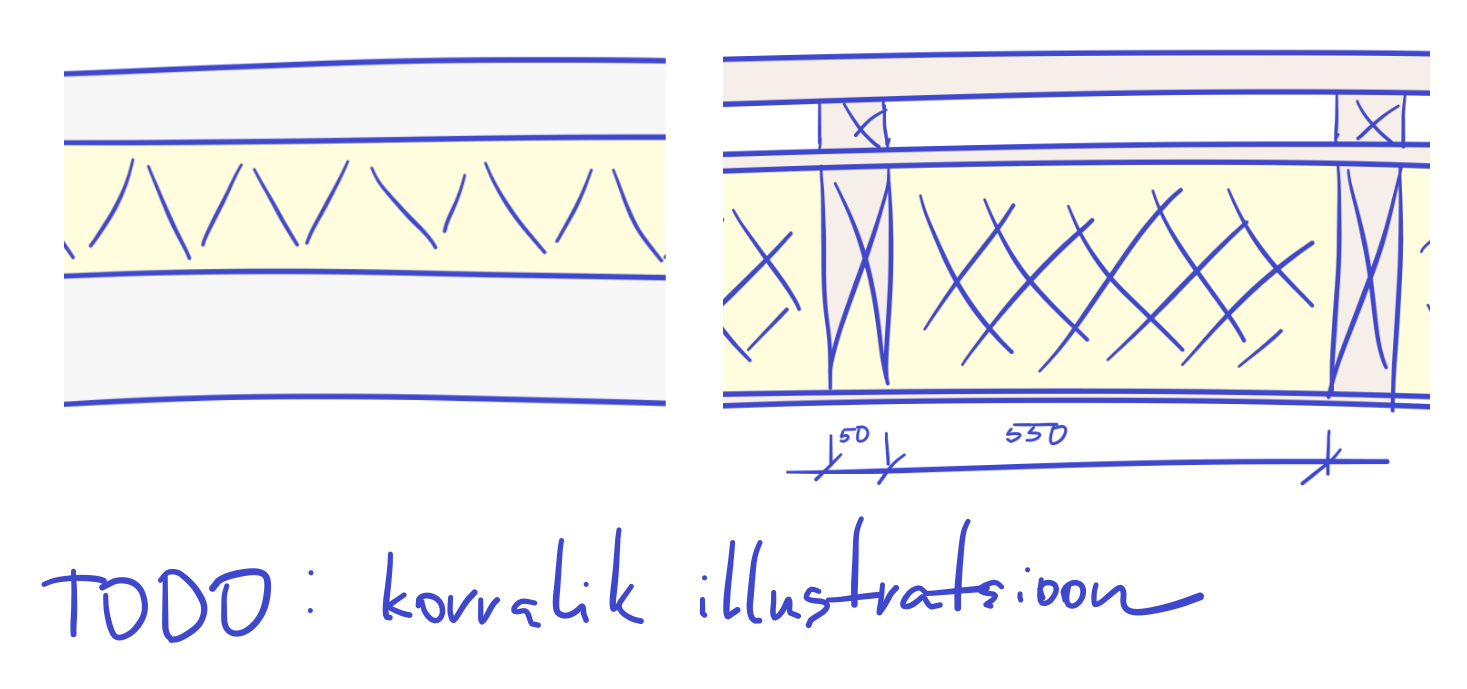
\includegraphics[width=.8\textwidth]{figures/problem_statement/06_un_non_unif_sample.png}
    \caption{\textit{Homogeense ja mittehomogeense konstruktsiooni näide}}
    \label{fig:construction_samples}
\end{figure}

Ehitusfüüsika seisukohalt kõige olulisemad materjali omadused on soojuserijuhtivus \begin{math}\lambda\end{math} [W/mK]
ja veeaurutakistus, mis võib olla väljendatud mitmel viisil (neid viise on palju, aga käesolevas töös keskendutakse 
ainult järgmistele, kuna need on kõige rohkem kasutatud nii raamatutes, kui ka materjalitootjate dokumentatsioonis):
\begin{math}\mu\end{math} - diffusioonitakistustegur (materjali omadus), Sd[m] - suhteline diffusioonitakistus (kindla paksusega toote omadus).


Kohalikul turul puudub tarkvara, millega oleks mugav teostada konstruktsiooni
 niiskustehnilise toimivuse analüüsi. Niiskustenilise toimivuse analüüs on klassikaline ehitusfüüsika ülesanne, mille 
 eesmärk on hinnata veeauru kondenseerumise (või ka kõrgest niiskusest põhjustatud kahjustuste tekkimise) riski.
Niiskustehnilise toimivuse analüüs hõlmab järgmisi tegevusi:
\begin{itemize}
    \item konstruktsiooni kihtide soojustakistuse ja konstruktsiooni summaarse soojustakistuse arvtus
    \item temperatuuri jaotuse määramine kihtides sõltuvalt sise- ja väliskeskkonna temperatuuridest ning 
    soojustakistuste väärtustest
    \item konstruktsiooni kihtide veeaurutakistuse ja konstruktsiooni summaarse veeaurutakistuse arvutus
    \item veeauru küllastusrõhu jaotuse määramine lähtuvalt temperatuuri jaotusest
    \item veeauru osarõhu jaotuse määramine kihides sõltuvalt sise- ja väliskeskkonna parameetritest ning 
    veeaurutakistuse väärtustest
    \item tulemuste esitamine graafiliselt diagrammil
    \item arvutuste kordamine erinevate sise- ja väliskeskkonna parameetrite kombinatsioonidega
\end{itemize}

Antud ülesannet lahendades käsitsi koostatakse tabelit, mille ridadele pannakse kirja kihid ja veergudele arvutatakse 
väärtused. Kuigi arvutused ei ole väga keerulised (tegemist on tavaliste füüsika valemitega), siis käsitsi arvutamine 
võtab tohutult palju aega. Kuigi Microsoft Excel võimaldab teatud määral protessi automatiseerida, siiski mõned 
tegevused (näiteks uue kihi lisamine) jäävad suures osas käsitööks, milles vea esinemine on väga tõenäoline. Pildil 
\ref{fig:excel_table_sample} on toodud sellise tabeli näide.
\begin{figure}[ht]
    \centering
    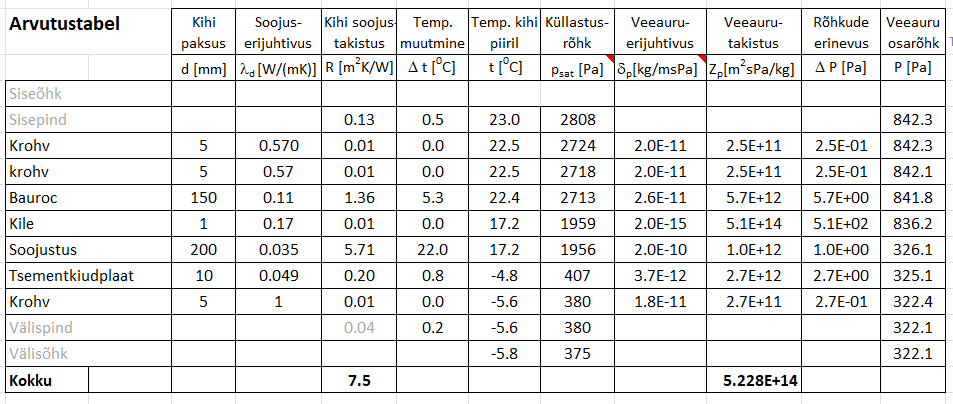
\includegraphics[width=.8\textwidth]{figures/problem_statement/04_calc_table.png}
    \caption{\textit{Niiskustehnilise toimivuse analüüsi tabeli näide}}
    \label{fig:excel_table_sample}
\end{figure}

Lõppkokkuvõttes analüüsi tulemused esitatakse graafiliselt diagrammi kujul, mille peale on kantud konstruktsiooni 
kihid, temperatuuri, veeauru küllastusrõhu ja veeauru osarõhu jaotuse graafikud (näide on toodud pildil \ref{fig:excel_graph_sample}). 
Selle tegevuse eesmärk on hinnata kondenseerumise riski konstruktsiooni kihtides. Veeauru osa- ja küllastusrõhu 
suhe on suhteline niiskus, vastavalt mida lähedam osarõhu graafiku joon küllasturõhu joonele -- seda kõrgem on 
antud konstruktsiooni kohas suhteline niiskus. Juhul kui mingis punktis osarõhu joon saavutab küllastusrõhu 
joont -- tekib selles punktis kondensaat. 

\begin{figure}[ht]
    \centering
    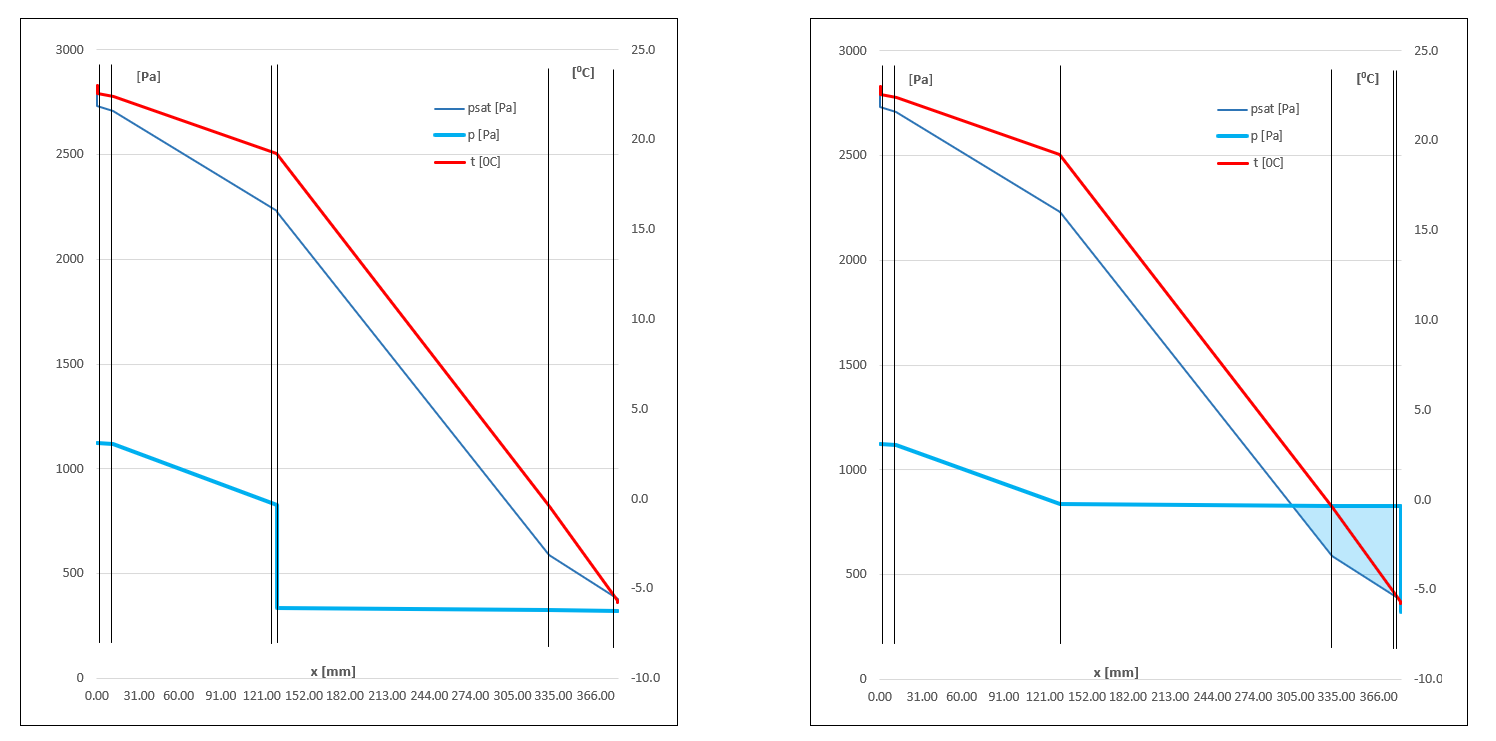
\includegraphics[width=.6\textwidth]{figures/problem_statement/05_excel_grafic_sample.png}
    \caption{\textit{Niiskustehnilise toimivuse analüüsi graafiku näide}}
    \label{fig:excel_graph_sample}
\end{figure}



\section{Olemasolevad lahendused ja turu analüüs}
Üks populaarsematest analoogidest, mida kasutatakse sealhulgas ka Eestis, on Saksa päritoluga tarkvara \textbf{Ubakus}. 
Tegemist on veebirakenduse kujul kommertstarkvaraga, mille \textit{demo}-versioon on saadaval tasuta (pilt \ref{fig:ubakus_sample}). 
\begin{figure}[ht]
    \centering
    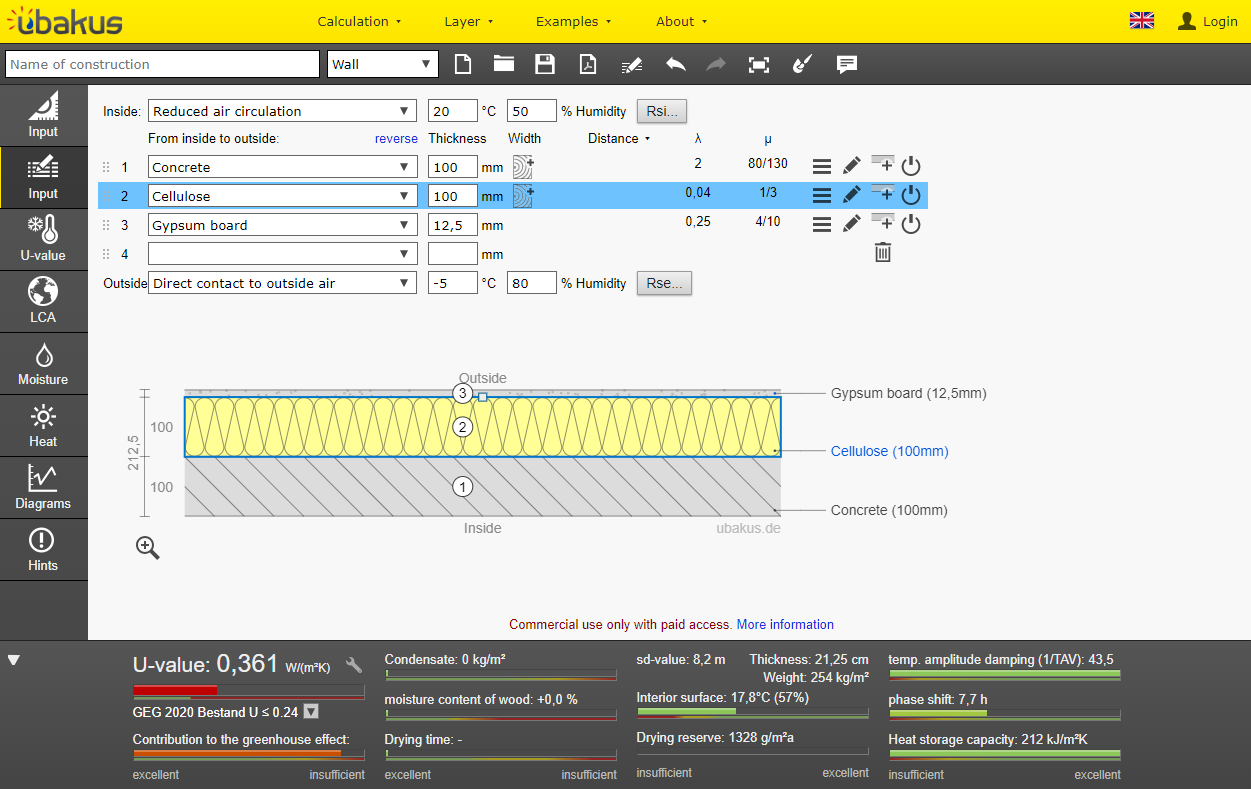
\includegraphics[width=.8\textwidth]{figures/problem_statement/01_ubakus.png}
    \caption{\textit{Ubakus veebirakenduse ekraanitõmmis.}}
    \label{fig:ubakus_sample}
\end{figure}

\textbf{Ubakus} võimaldab teostada konstruktsiooni niiskustehnilist analüüsi. Kasutajaliides võidaldab 
mudeldada mitmest kihist koosneva konstruktsiooni, valides igale kihile paksust ja materjali, millest 
kiht koosneb. Tugev eelis on see, et tarkvaraga saab analüüsida ka mittehomogeensete (mitemest erinevast 
materjalist, nt puitsõrestiksein) kihtidega konstruktsioone - pilt \ref{fig:ubakus_layers}

\begin{figure}[ht]
    \centering
    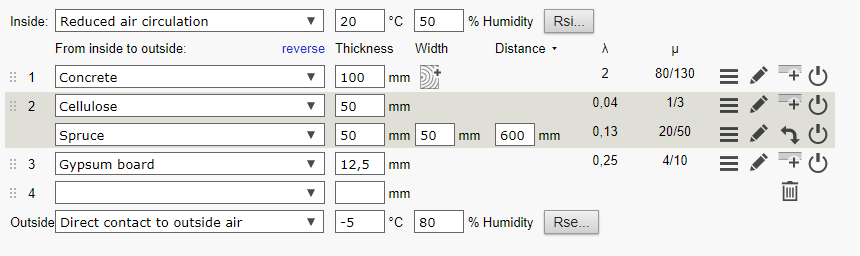
\includegraphics[width=.6\textwidth]{figures/problem_statement/02_ubakus_layers.png}
    \caption{\textit{Ubakus: konstruktsiooni kihtide lisamine.}}
    \label{fig:ubakus_layers}
\end{figure}

Ehitusmaterjalide valik, mida on võimalik konstruktsiooni mudeldamisel kasutada, on piisavalt lai 
(aga tasuta versioonis piiratud). Tasulises versioonis on samuti võimalik ka oma materjalide 
lisamine ja kasutamine. Puuduseks on see, et teatud osa baasis olevatest ehitusmaterjalidest on Saksamaal
turustatavad materjalid, mistõttu selle tarkvara kasutades Eestis peab kas sisestama kõik vajalikud 
materjalid käsitsi, või kasutada Saksa analoogid ning arvestada sellest tulenevaarvutuste ebatäpsusega.
\begin{figure}[ht]
    \centering
    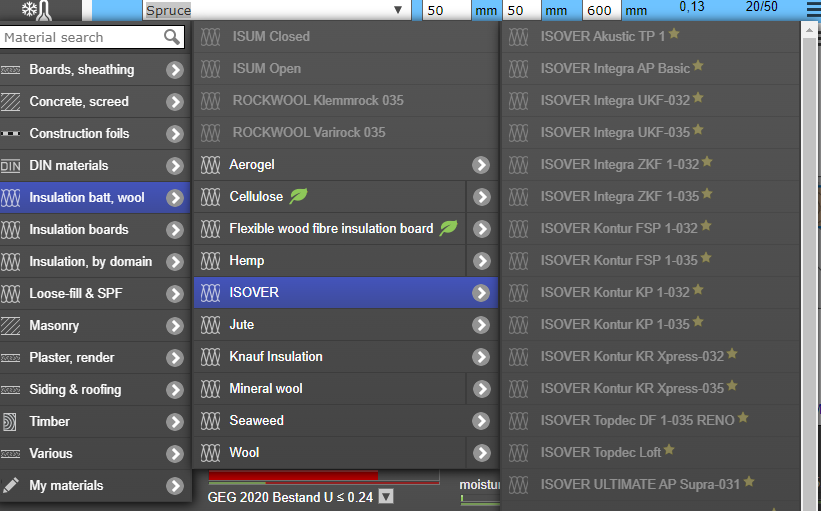
\includegraphics[width=.6\textwidth]{figures/problem_statement/03_ubakus_materials.png}
    \caption{\textit{Ubakus: ehitusmaterjalide valik baasis.}}
    \label{fig:ubakus_materials}
\end{figure}


\chapter{Kavandatava veebirakenduse analüüs}\label{chapter:analysis}
\section{Nõuete defineerimine}
\label{chapters:analysis_requirements}
\subsection{Funktsionaalsed nõuded}
\label{subsec_func_req}
Funktsionaalsete nõuete määramisel lähtutakse erinevate osapoolte vajadusest - süsteemi kasutaja ja süsteemi 
administraator. Nõuete sõnastamisel on aluseks töö autori isiklik kogemus ja teadmised sihtgrupi vajadustest ja nõuetest.

\textbf{Infosüsteemi kasutajal peab olema võimalus:}
\begin{itemize}
    \item registreerida endale konto ja logida sisse
    \item hallata oma konto andmeid
    \item tellida tasulist paketi
    \item vaadata enda poolt salvestatud materjalide nimekirja
    \item luua ja salvestada uus materjal
    \item redigeerida varem salvestatud materjal
    \item kustutada varem salvestatud materjal
    \item lisada uus kiht konstruktsiooni mudelisse
    \item valida uue kihi materjal
    \item sisestada uue kihi paksuse väärtust
    \item redigeerida olemasolevat kihti
    \item kustutada olemasolevat kihti
    \item vahetada kihtide järjekorda
    \item valida välistingimuste parameetrid
    \item valida sisetingimuste parameetrid
    \item valida konstruktsiooni tüüp
    \item vaadata tulemusi tabeli kujul (valikuliselt)
    \item vaadata tulemusi graafikul (valikuliselt)
    \item vaadata konstruktsiooni toimivuse mõõdikuid
    \item peale igat muutust kohe näha uusi tulemusi (arvulised väärtused)
    \item peale igat muutust kohe näha graafikute uuendamist
    \item näha konstruktsiooni skemaatilist joonist
    \item salvestada mudeldatud konstruktsiooni
    \item vaadata salvestatud konstruktsioonid
    \item kustutada salvestatud konstruktsioonid
    \item avada salvestatud konstruktsioonid kalkulaatoris
    \item muuta kiht mittehomogeenseks
    \item mittehomogeensele kihile lisada alamkihid
    \item valida alamkihtide materjalid
    \item sisestada alamkihtide paksuse väärtust
    \item näha konstruktsiooni skemaatilist joonist
    \item näha skemaatilise joonise peal graafikut
    \item näha skemaatilise joonise peal värvilist temperatuurikaarti
    \item näha dünaamilist analüüsi aasta lõikes
    \item valida kliimaandmeid dünaamilise analüüsi jaoks
    \item genereerida analüüsi aruanne PDF formaadis
\end{itemize}



\textbf{Infosüsteemi administraatoril peab olema võimalus:}
\begin{itemize}

    \item vaadata kasutajate nimekirja
    \item hallata kasutajaid
    \item seadistada tellimust vormistanud kasutajale vastavad õigused
    \item hallata kasutajate andmeid
    \item vaadata süsteemis salvestatud vaikimisi materjalide nimekirja
    \item salvestada uus materjal
    \item määrata materjali ligipääsu taset
    \item redigeerida varem salvestatud materjal
    \item kustutada varem salvestatud materjal
    \item hallata uusi materjali kategooriaid
    \item hallata uusi materjalide tootjaid
    \item hallata keskkonna seadistuse valikuid
    \item lisada kliimaandmeid failina
\end{itemize}

Funktsionaalsest nõuetest on kokku pandud kasutajalood, mis omakorda jagatud featuurideks. Protsessi visualiseerimiseks on kasutatud Miro interaktiivne
keskkond. Kliendi kasutajalood on jagatud kuueks featuuriks (pilt \ref{fig:client_userstories}):
\begin{itemize}
    \item infosüsteemi kasutamine
    \item ehitusmaterjalide andmebaasi haldamine
    \item konstruktsiooni mudeldamine
    \item arvutuse lisatingimuse seadistamine
    \item analüüsi tulemuste esitamine
    \item salvestatud konstruktsioonide haldamine
\end{itemize}

Administraatori kasutajalood on jagatud kolmeks featuuriks (pilt \ref{fig:admin_userstories}):
\begin{itemize}
    \item infossteemi kasutajate haldamine
    \item ehitusmaterjalide avaliku andmebaasi haldamine
    \item lisaandmete baasi haldamine
\end{itemize}

Samuti olid kasutajalood kategoriseeritud prioriteedi järgi. Kõrgema prioriteediga kasutajalood moodustavad MVP funktsionaalsust, mida arendatakse käesoleva lõputöö käigus.
Osa funktsionaalsusest, mis on kirjeldatud madala prioriteedi kasutajalugudega, jääb käesoleva lõputöö skoobist välja. Suures osas see puudutab tulemuste esitamise
viise: mudeldatud konstruktsiooni skemaatilise 2D joonise genereerimine ning selle peale graafikute või värvikaartide pealekandmine eeldab 
eraldi teeki kirjutamist. Isegi kui värvikaartide puhul õnnestuks leida valmislahendust, siis selle adapteerimine siiski tähendab suurt töömahtu.
Samuti on MVP skoobist välja jäetud mittehonogeensete kihtidega konstruktsioonide arvutus. Andmemudelid kohe tuleb projekteerida nii, et tulevikus
see oleks võimalik implementeerida ilma suurte muutusteta , kuid arvutuste ja kasutajaliidese lihtsustamise mõttes jääb see osa esimese iteratsiooni skoobist välja.


\begin{figure}[ht]
    \centering
    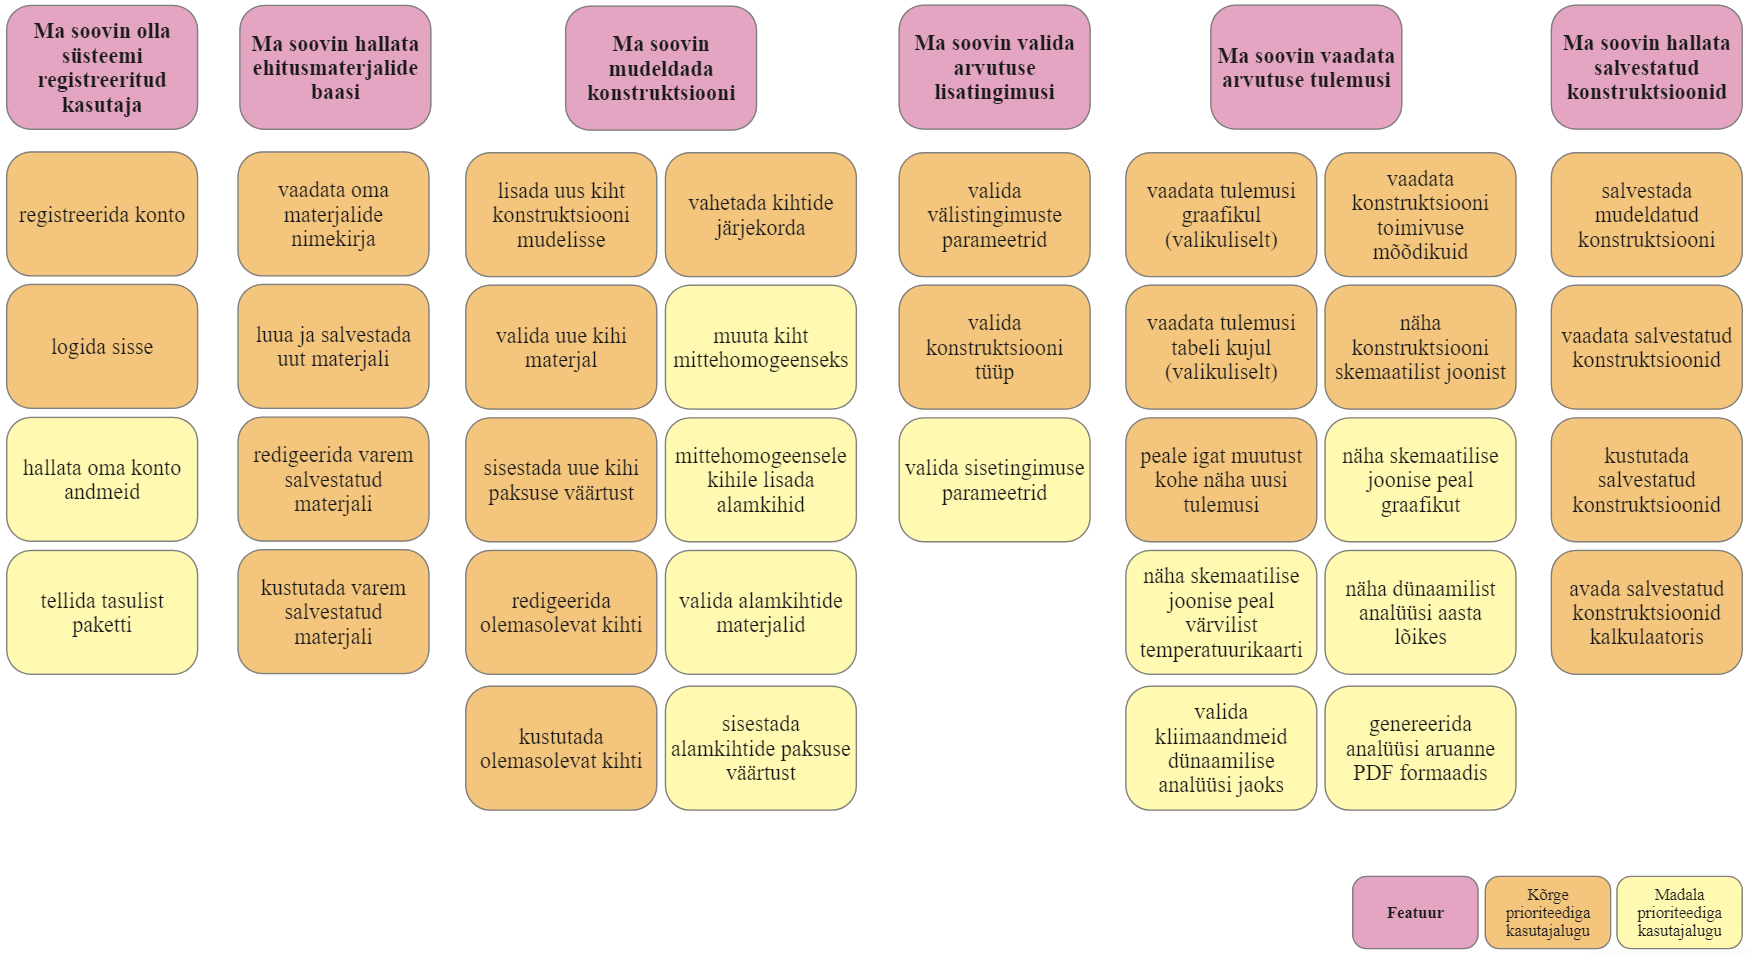
\includegraphics[width=1\textwidth]{figures/analysis/client_userstories.png}
    \caption[Funktsionaalsed nõuded, kliendi kasutajalood]{\textit{Kliendi kasutajalood}}
    \label{fig:client_userstories}
\end{figure}

\begin{figure}[ht]
    \centering
    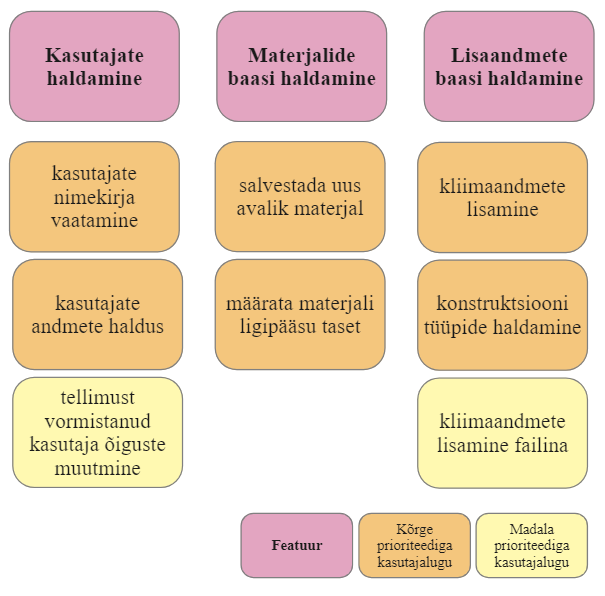
\includegraphics[width=0.6\textwidth]{figures/analysis/admin_userstories.png}
    \caption[Funktsionaalsed nõuded, administraatori kasutajalood]{\textit{administraatori kasutajalood}}
    \label{fig:admin_userstories}
\end{figure}

\subsection{Mittefunktsionaalsed nõuded}
Lisaks osas \ref{subsec_func_req} kirjeldatud funktsionaalsetele nõuetele, peab süsteem vastama järgmistele nõuetele:
\begin{itemize}
    \item kasutajaliides peab olema kiire -- kasutaja peab nägema arvutuse tulemuste uuendamist kohe peale 
lähteandmete (kihid, parameetrid) muutmist, pikk ooteaeg või lehe ümberlaadimine tulemuste näitamiseks ei ole aktsepteeritav;
    \item kasutajaliides peab olema kasutajasõbralik -- kasutaja peab intuitiivselt aru saama, mida ta peaks tegema, et 
jõuda tulemuseni, vajadusel peab ta olema juhitud \textit{popup}-tüüpi infoplokidega;
    \item kasutajaliides peab olema kaasaaegne, st välimus ja veebilehe struktuur peavad
vastama kaasaaegsetele UX/UI printsiibidele.
\end{itemize}

\section{Tehnoloogiate valik}
Tehnoloogiate valimisel lähtutakse kaasaaegsetest veebirakendamise ehitamise pritsiibidest, arvestatakse
rakenduse loogika keerukust, võimalike kasutajate hulka, säilitavate andmete mahtusid ja infosüsteemi
edasise arengu perspektiive. 

Veebirakendusel peab olema selgelt eristatav serveriosa ja kasutajaliides. Vajadusel saab tulevikus 
implementeerida ka teised kasutajaliidesed, mis töötavad sama serveriosaga (näiteks: mobiilrakendus).
See tähendab, et infosüsteemi arhitektuur peab olema REST arhitektuurse stiili nõuete kohane. See eeldab
ka seda, et andmevahetus kasutajaliidese ja serveriosa vahel peab toimuma HTTP päringutega kasutades 
JSON (JavaScript Object Notation) formaati. JSON on JavaScript-i põhine andmevahetuse formaat, mis 
representeerib JavaScript-i andmeobjektid tekstilisel kujul, mida on võimalik saata HTTP 
päringutega üle veebi\cite{about_rest}.
Lisaks sellele on oluline, et kõik päringud on omavahel sõltumatud, see tähendab, et ühe 
päringu raames serveriosas alustatakse ja lõpetatakse kõik päringuga seotud protsessid, päringute 
vahel serveril puudub kliendiga seotud olek (\textit{stateless} protokoll)\cite{about_rest}.

Selleks, et süsteem saaks võimalikult pikemat aega töötama ilma tehnoloogiate uuenduse vajaduseta,
peab kasutusele võtma võimalikult uued, aga samas ka stabiilsed ja pikema toega lahenduste versioonid. 
 

\subsection{Kasutajaliides}
\label{analysis_interface_subsection}
Kasutajaliides implementeeritakse üheleherakendusena (SPA). SPA tehnoloogia võimaldab minimeerida 
andmevahetuse mahtusid: serverilt küsitakse ja vastavalt kliendile saadetakse ainult need andmed, 
mida on hetkel tarvis. Arendatava infosüsteemi kontekstis see on oluline, sest kõiki arvutusi 
teostatakse serveril ning kliendile saadetakse andmed, mis on vajalikud tulemuste näitamiseks 
kasutajale. Iga uus tegevus kasutajaliideses, mis mõjutab tulemusi (uue kihi lisamine, 
kihtide järjekorra muutmine, arvutuse parameetrite muutmine jms.), tähendab uut päringut serverile. 
Samuti SPA tehnoloogia võimaldab muuta lehe sisu dünaamilisel viisil -- uuendatakse vaid lehe teatud
komponent ilma kogu lehekülje ümberlaadimise vajaduseta \cite{about_spa}. See on ka oluline, kuna tulemuste esitamist 
peab uuendama dünaamiliselt kohe peale arvutuse lähteandmete muutmist.

Üheleherakenduste implementeerimiseks kasutatakse JavaScript programmeerimiskeelt veebilehe dünaamilise 
loogika juhtimiseks. Soovitavalt kasutada JavaScript keele laiendust -- TypeScript, mis muudab JavaScript-i 
tugevalt ja staatiliselt tüübitud keeleks \cite{about_typescript}. Lehtede struktuuri ehitamiseks kasutatakse HTML (või raamistikust
sõltuv laiendatud HTML-i süntaks). Kujundust teostatakse CSS stiilireeglitega ja lihtsustamise mõttes
võetakse kasutusele ka vastavad teegid nt Bootstrap.

Kuigi on võimalik implementeerida loogikat kasutades puhtat JavaScript koodi, tänapäeval seda tehakse
harva. On olemas erinevad lahendused, mis oluliselt lihtsustavad rakenduse ehitamise protsessi, kuid 
nõuavad ka spetsiifilisi teadmisi. Raamistiku kasutuselevõtt olulisel määral vähendab koodi kirjutamist,
kuna raamistik ise haldab loogikat, mis on seotud näiteks \textit{Routing}-uga, turvalisusega, komponentide
genereerimise ja uuendamisega. Spetsiifilise funktsionaalsuse jaoks kasutatakse eraldi pluginaid ja teeke. Näiteks
päringute saatmise ja serveri vastuse töötluseks kasutatakse \textit{Axios} -- teek, mida saab kasutada 
erinevate raamistikutega.

Üheleherakenduse implementeerimiseks kõige sobilikud JavaScript raamistikud on \textit{React}, \textit{Vue.js}
ja \textit{Angular}. Kõikidel raamistikutel on oma eripärad alates projekti arhitektuurist kuni 
koodi süntaksini. 

\textit{React} on laialt levinud \textit{front-end} teek, mis kasutab JavaScript programmeerimiskeelt. 
Lehe šablooni kujundamiseks kasutatakse JSX (JavaScript XML). JSX on JavaScript-i laiendus, mis võimaldab
sisestada HTML koodi JavaScript-i programmi. Rakendus koosneb React-elementidest, mille oleku haldamisega teek
tegeleb ise. Elemendid on taaskasutatavad ning nendele antakse andmeid edasi andmeobjektide kujul (\textit{props}).
Kuna lahendus on populaarne -- selle kasutamise kohta on kogutud palju teavet ja kogemust veebis, mistõttu
probleemide tuvastamine ja lahenduste leidmine on piisavalt lihtne. Lisaks sellele eksisteerib palju pluginaid
ja teeke, mida saab React raamistikuga ühendada funktsionaalsuse laiendamiseks. 

\textit{Vue.js} on MVVM (Model-View-ViewModel) tüüpi raamistik. Lehe šablooni kujundamiseks kasutatakse HTML, 
mis siseldab Vue-spetsiifilist süntaksi, mille abil juhib raamistik lehe logikat. Vue rakendus koosneb SFC 
komponentidest, igas komponndis on eraldi defineritud lehe šabloon, skript ja stiil. Vue.js raamistik on
samuti laialt levinud ja selle kohta on võimalik Internetist piisavalt infot leida.

\textit{Angular} on MVC (Model-View-Controller) tüüpi raamistik. Angular-i projekt struktuurselt koosneb
moodulitest, komponentidest ja teenustest. Angular-is kasutatakse lehe šabloonides sarnaselt Vue raamistikule
HTML koodi Angular-spetsiifilise süntaksiga. 

Kõik ülaltoodud raamistikud toetavad ka \textit{TypeScript}-i kasutamist. Oma funktsionaalsuse seisukohalt
kõik toodud raamistikud võimaldavad implementeerida kavandatavat funktsionaalsust (\textit{routing}, 
oleku juhtimine, komponentide dünaamiline uuendamine), seega määravaks asjaoluks on arendamisega tegeleva 
programmeerija eelistused. Kuigi töötamise kiirus on raamistikutel erinev, planeeritava rakenduse suurusjärgu
kontekstis see faktor ei ole kriitiline. 

Toodud põhjendustel valitakse kasutajaliidese tehnoloogiaks React-i. Programmeerimiskeeleks peab valima TypeScript, 
mis on erinevalt JavaScript-ist võimaldab teha tüübikirjeldust, tänu millele on programmi käitumine ettearvatavam, 
vigade tõenäosus väiksem ja kood on üldiselt kvaliteetsem. React on populaarne lahendus, seetõttu eksisteerib palju
teeke, pluginaid ja leindusi, mida tõneäoliselt saab kasutusele võtta. Kasutada peab React viimane versioon,
mis on käesoleva töö koostamise hetkel v18.2.


\subsection{Serveriosa}
\label{analysis_backend_subsection}
Serveril töötav \textit{backend} rakendus tegeleb kasutajaliidese päringute töötlusega ja andmete saatmisega.
Samuti \textit{backend} osa suhtleb andmebaasiga, küsides ja redigeerides andmeid. Rakenduse serveriosa on võimalik
implementeerida kasutades järgmiseid programmeerimiskeeli:
\begin{itemize}
    \item \textit{PHP} -- popupaarne ja ka võrdlemisi lihtne programmeerimiskeel (avaldatud 1995. aastal), 
    mille otstarve oli kohe alguselt suunatud veebilehtede ehitamiseks. Kuigi esialgu PHP kontseptsioon oli selline, 
    et HTML-kood genereeriti serveril ja saadeti veebilehitsejale iga kord uuesti näitamiseks (monoliitne arhitektuur), 
    siis viimasel ajal kastutakse PHP ka REST-tüüpi veebirakendustes, kus serveril töötav PHP programm saadab 
    andmeid kasutajaliidese rakendusele JSON (või muul) kujul. Tugevaks eeliseks on see, et suur osa veebimajutust 
    pakkuvaid teenuseid toetavad täna PHP keelt vaikimisi, mistõttu rakenduse paigaldamise protsess sellisel juhul 
    on oluliselt lihtsam (koondub programmi failide kopeerimisele serverile).
    \item \textit{Java} -- objektorienteeritud programmeerimiskeel (avaldatud 1995. aastal), mille arendamisega 
    tegeleb Oracle. Keel sobib suuremate REST-tüüpi veebirakenduste ehitamiseks, kuid selle kasutusvaldkond on palju laiem kui 
    ainult veebirakendused. Java on tugevalt ja staatiliselt tüübitud keel, mis on suureks eeliseks, kuna alandab
    vigade tekkimise tõenäosust, lisaks on see piisavalt kiire.  Samas eeldab see spetsiifilisi teadmisi 
    programmeerialt ja ka rakenduse paigaldamine serverile on erinevalt PHP-st ka keerulisem, kuna projekti 
    ehitamine eeldab palju lisategevusi. Java on kasutusel väga suure kasutajate hulgaga infoüsteemides (sh. ka pangasüsteemid).
    \item \textit{C\#} -- objektorienteeritud programmeerimiskeel (avaldatud 2000. aastal), mille arendamisega tegeleb Microsoft. 
    Keele süntaks ja programmi struktuuri põhimõtted on väga sarnased Java-le. Keel on tugevalt tüübitud ja 
    ka programmi struktuur on Java-keelega analoogne. C\# samuti sobib suurte infosüsteemide ehitamiseks.
    \item \textit{Python} --  üldotstarbeline programmeerimiskeel, mille kasutusvaldkond on lai -- programmeerimise 
    õpetamist koolilastele kuni suurte infosüsteemide ehitamiseni -- tänu kõigepealt sellele, et keele süntaks on 
    võrdlemisi lihtne ning vastavalt keel on kergemini õpitav. Keel on dünaamiliselt tüübitud, mida erinevates s
    ituatsioonides saab pidada nii eeliseks kui ka puuduseks.
\end{itemize}

Rakenduse ehitamiseks on otstarbekas kasutada analoogselt kasutajaliidesega raamistikku. Kõikidel ülaltoodud
programmeerimiskeeltel eksisteerivad raamistiku lahendused, mis sobivad veebirakenduse serveriosa ehitamiseks.

\begin{itemize}
    \item \textbf{Laravel} - PHP keeles kirjutatud raamistik, väga populaarne ja laialt levinud, funktsionaalsus 
    katab kõiki veebirakenduse ehitamise vajadusi.
    \item \textbf{Spring} - Java keeles kirjutatud raamistik veebirakenduse ehitamiseks. Sisaldab palju erinevaid 
    mooduleid (nt Spring Security - turvalisust tagav raamistiku osa, Spring MVC - MVC raamistik jm), mis 
    tervikuna moodustavad tugevat infrastruktuuri suurte infosüsteemi ehitamiseks.
    \item \textbf{.NET} - C\# keeles raamistik, mis samuti sobib REST veebirakenduste ehitamiseks. 
    Vajalik funktsionaalsus on tagatav vastavate paketide paigaldamisega (nt EntityFrameworkCore - 
    ORM raamistik, AspNetCore.Authentification.JwtBearer - JWT tokeni kaudu autentimise võimaldamine).
    Viimastel aastatel on raamistiku populaarsus oluliselt vähenenud.
    \item \textbf{Django} - Python keeles kirjutatud raamistik. On lihtne ja laia funktsionaalsusega,
    mis on kohe raamistikus saadaval ilma lisamoodulite paigaldamise vajaduseta.
\end{itemize}

Arendatava infosüsteemi seisukohalt peab tehnoloogia sobivuse hindama järgmiste aspektide seisukohalt: 
\begin{itemize}
    \item kiirus -- teenus peab piisavalt kiiresti teostama kõikvõimalikud arvutused, sh kasutades samal
    ajal andmeid andmebaasist.
    \item turvalisus -- raamistik peab (sisseehitud funktsionaalsus või laiendus) tegelema
    rakenduse turvalisusega sh kasutajate autentimisega. Raamistik peab toetama ka JWT tokeniga
    autentimist.
    \item ORM -- raamistikul peab olema \textit{Object Relational Mapping}-uga tegelev moodul, 
    selleks et lihtsustada andmebaasi andmetega tegutsemist koodis.
    \item arendaja oskused -- infosüsteemi arendamisega tegeleval ressurssil peavad olema piisavalt teadmisi
    ja kogemusi raamistikuga
\end{itemize} 

Raamistikute vastavus eeltoodud kriteeriumitele on toodud tabelis \ref{tab:requirements}.
\begin{longtable}{|p{3cm}|p{2.5cm}|p{2.5cm}|p{2.5cm}|p{2.5cm}|}
	\caption{\it{Backend raamistikute võrdlus}}
	\label{tab:requirements}\\ \hline
	\textbf{Raamistik} &  \textbf{Kiirus} & \textbf{Turvalisus}  & \textbf{ORM} & \textbf{Oskused} \\
	\hline
	\endhead
	\endfoot
	\hline
	\endlastfoot
Laravel & + & + & + & +/-  \\ \hline
.NET    & + & + & + & +  \\ \hline
Spring  & + & + & + & +/-  \\ \hline
Django  & + & + & + & -  \\ \hline
\end{longtable}

Kõik raamistikud omavad vajalikku funktsionaalsust arendatava infosüsteemi ehitamiseks, seetõttu valiku tegemist 
lähtutakse saadaval oleva programmeerimisressurssi oskuste tasemest erinevate raamistikutega. Sellest lähtuvalt
oli tehnoloogiaks valitud C\# keeles kirjutatud .NET raamistik.

\subsection{Andmebaasi juhtprogramm}
\label{analysis_database_subsection}
Kuna inosüsteemi äriloogika ei eelda suurte andmete mahtude säilimist, seetõttu ka andmebaasi juhtsüsteemi 
valiku osas on nõuded tagasihoidlikud: \textit{Open Source} tüüpi litsents, et välistada lisakulusid ning
võimalus ühendada andmebaasimootor valitud serveriosa raamistikuga (.NET). Kõige populaarsemad 
\textit{Open Source} litsentsiga andmebaasimootorid on:
\begin{itemize}
    \item MySQL
    \item PostgreSQL
    \item MariaDB
    \item MongoDB
    \item SQLite
\end{itemize}
Kõikidele ülaltoodud süsteemidele eksisteerivad juhtprogrammid .NET EF Core ühendamiseks, seetõttu võib kõik
toodud lahendused pidada sobilikuks. Valikul lähtutakse sellest, mis tehnoloogiaga on programmerijal rohkem teadmisi 
ja kogemusi. Antud juhul see on PostgreSQL. 


\section{Veebirakenduse arhitektuur}
\label{chapters:analysis_architecture}
Kavandatava infosüsteemi komponendid on järgmised:
\begin{itemize}
    \item \textbf{server} -- renditud pilveserver Ubuntu 20.04 operatsioonisüsteemiga
    \item \textbf{back-end} -- infosüsteemi serveriosa .NET 8.0.1, käivitatud Docker-konteinerina serveri operatsioonisüsteemis
    \item \textbf{front-end} -- serveri kasutajaliidese osa React v18.2
    \item \textbf{andmebaas} -- andmete salvestamiseks, andmebaasimootor PostgreSQL 16.2 paigaldatakse sama pilveserveri operatsioonisüsteemile
\end{itemize}

\begin{figure}[ht]
    \centering
    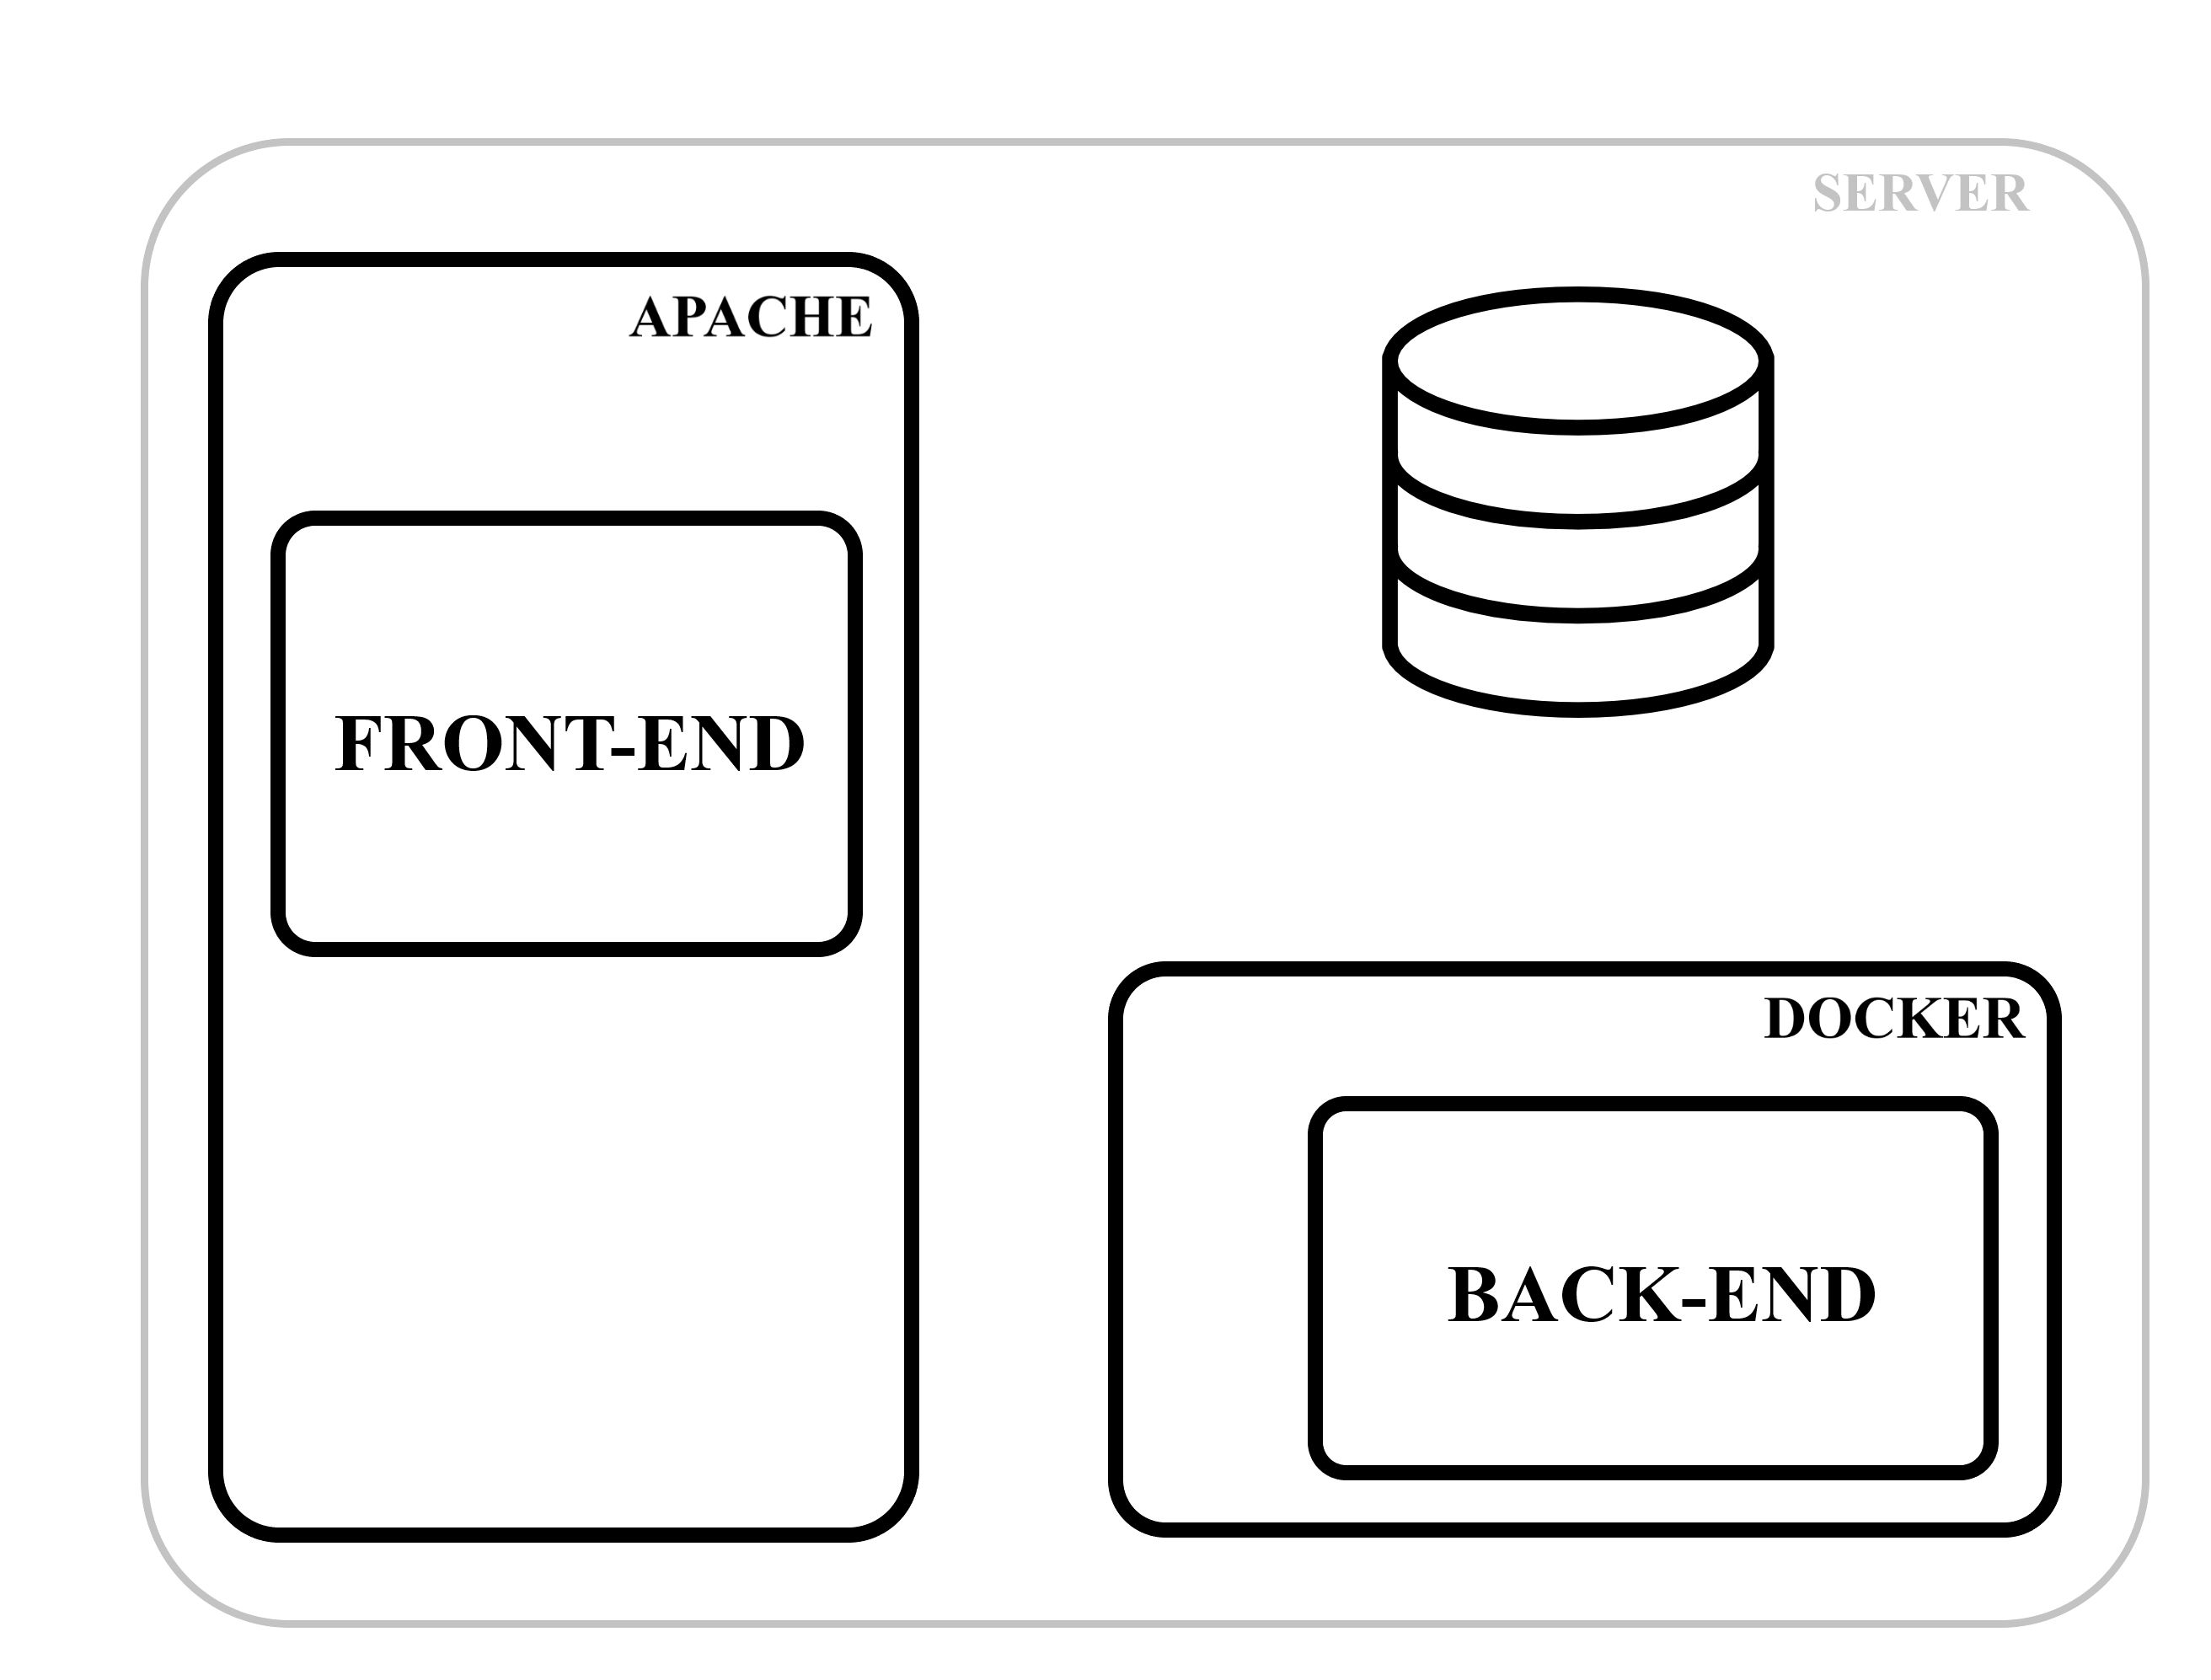
\includegraphics[width=0.9\textwidth]{figures/analysis/architecture.png}
    \caption[Infosüsteemi arhitektuur]{\textit{Infosüsteemi arhitektuur}}
    \label{fig:architecture}
\end{figure}

Infosüsteemi komponentide omavahelised seosed on toodud Joonisel \ref{fig:architecture}.
Pilveserveri teenuse rentimise valikult tuleb kindlasti arvestada, et teenus peab võimaldama operatsioonisüsteemi
haldamist \textit{root}-kasutajana, et oleks võimalik Docker-i kaudu käivitada rakenduse serveriosa ning
paigaldada PostgreSQL andmebaasimootor. Samuti tuleb paigaldada Apache server, mis hakkab 
serveerima kasutajaliidese rakendust ning edastada teatud aadressile tulnud päringud (\textit{reverse proxy})
Docker-konteineris töötavale \textit{backend}-rakendusele.


\section{Andmebaasi projekteerimine}
Osa, kus käsitletakse andmebaasi projekteerimist.

\section{Kasutajaliidese disain}
Osa, kus käsitletakse kasutajaliidest ja selle kavandamist

\chapter{Veebirakenduse arendus}\label{chapter:development}
Veebirakenduse arendamise osa
\section{Andmebaas}
Vastavalt käesoleva töö osale \ref{analysis_database_subsection} projekti realiseerimiseks
on valitud PostgreSQL versioon 16. Andmebaasi juhtprogramm paigaldatakse samale serverile, milles 
käivitatakse ka ülejäänud infosüsteemi osad. PostgreSQL on Ubuntus paigaldamiseks saadaval
\textit{apt} repositooriumil. Peale paigaldamist redigeeritakse PostgreSQL konfiguratsiooni - 
\textit{postgresql.conf} ja \textit{pg hba.conf}, seadistades porti, mida kuulatakse (5432) ning 
IP aadressid, millistelt võetakse päringuid vastu.

Turvalisuse tagamiseks luuakse arendatavale rakendusele eraldi PostgreSQL kasutajat parooliga, 
piirates kasutaja õigusi ühe konkreetse andmebaasiga, mis on rakenduse funktsioneerimiseks tarvis.
Andmebaasile tehakse iganädalased varukoopiad, mida salvestatakse serveril. Selle jaoks luuakse skripti ning 
määratakse Ubuntu Cron regulaarse tööna.




\section{Serveriosa}
Serveriosa arhitektuur on kihiline -- andmete töötlus alates andmebaasist küsimisest kuni kasutajale saatmiseni toimub neljas kihis:
\begin{itemize}
    \item andmebaasi ja domeeni kiht,
    \item andmete ligipääsu kiht,
    \item äriloogika kiht,
    \item andmete representeerimise kiht.
\end{itemize}
Kihtide eesmärk on selgelt eristada andmete töötlust loogika ja otstarve järgi. Andmete representeerimise kiht tegeleb andmete 
kasutajaliidesele saatmise ja kasutajaliideselt vastuvõtmisega ning ei pea muretsema sellest, mis toimub andmetega äriloogika kihis. 
Analoogselt ka andmete ligipääsu DAL kihis teostatakse ainult andmete küsimist ja salvestamist andmebaasile
(antud töö raames -- raamistiku kaudu), võimalikult välistades igasugused infosüsteemi äriloogikaga seotud tegevused. 
Kihid on näidatu Joonisel \ref{fig:development_backend_layers}.

\begin{figure}[ht]
    \centering
    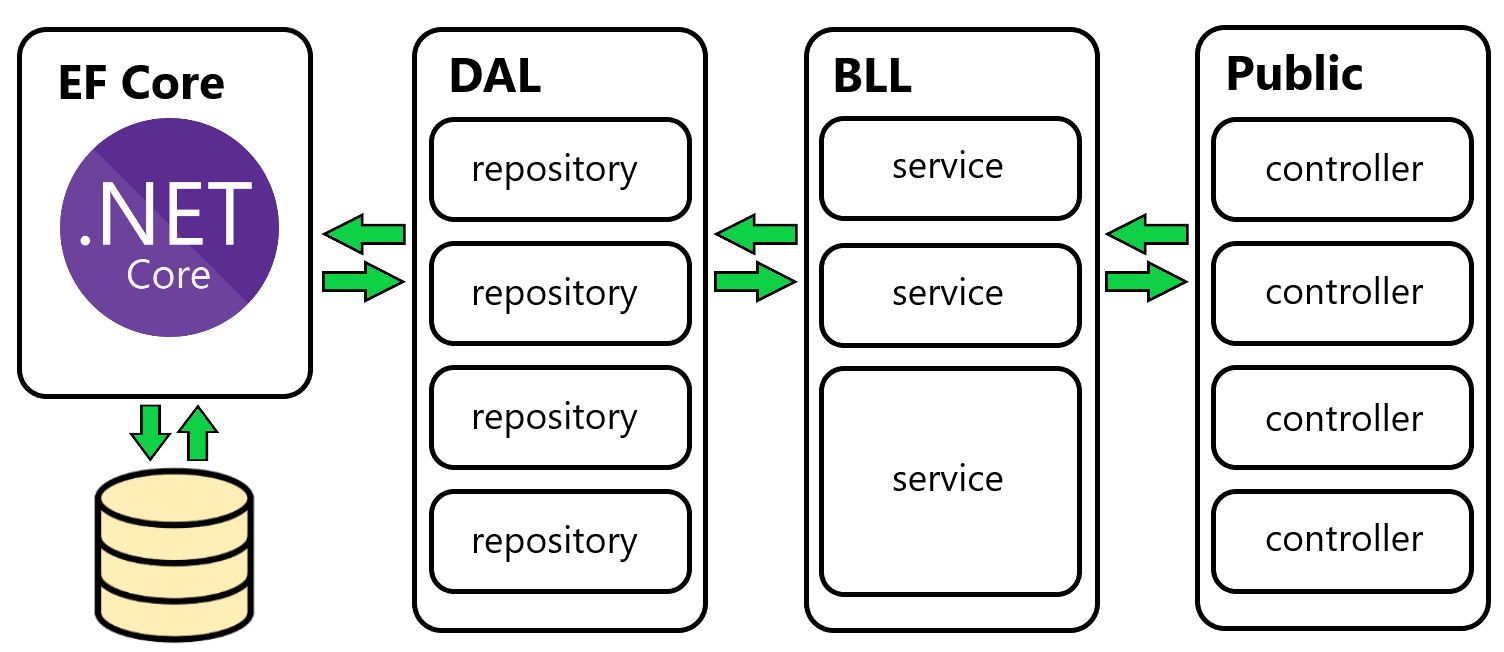
\includegraphics[width=1\textwidth]{figures/development/backend_structure.png}
    \caption[Serveriosa kihtide skemaatiline joonis]{\textit{Serveriosa kihtide skemaatiline joonis}}
    \label{fig:development_backend_layers}
\end{figure}
 

\textbf{EF Core} ja \textbf{Domain} kihis realiseeritakse projekteeritud andmebaasi mudel vastavate klassidena (näiteks \textit{Domain.App.Material},
\textit{Domain.App.Material-Category}, \textit{Domain.App.Material-Property} jne). Igas klassis määratakse olemitele vajalikud omadused ja
olemite vahelised seosed. Domeeni kiht moodustab andmebaasi konteksti (\textit{DbContext}), mis on \textit{Entity Framework Core} raamistiku klass,
mille kaudu raamistik suhtleb andmebaasiga. Raamistiku kaudu luuakse andmebaasi genereerimise ja uuendamise skripte - migratsioonid
(\textit{migration}). Kui üks olemite klassidest oli muudetud, siis uue migratsiooni tegemisel 
võrdleb raamistik uut olekut eelmisega ning genereerib uue skripti.


\textbf{DAL} andmete ligipääsu kihis teostatakse tööd andmebaasi konteksti  objektiga (DbContext):  andmeid küsitakse Entity Framework Core-ist ja 
vastavalt ka salvestatakse \textit{DbContext}-isse. Kiht on jagatud üksusteks -- repositooriumideks (\textit{Repository}), mis on 
baasimplementatsioonis kujutavad ennast klassikalist CRUD-tüüpi repositooriumit. Samuti repositooriumis 
tehakse  andmetele ligipääsu kontrolli kasutaja ID alusel -
nt meetod \textit{GetAllAsync(Guid uid, bool includePublic = false)} vaikimisi küsib andmebaasist kõik olemid, 
mis kuuluvad kasutajale ID-ga \textit{uid} ning valikuliselt lisatakse ka olemeid, mis on ette nähtud ühiskasutuseks. 
\textbf{TODO: Repositooriumi näidiskood, töö Lisa X}

Repositooriumiteks jagamist teostatakse andmemudeli ülesehituse alusel -- iga olemi jaoks on eraldi repositoorium. Selleks, et
äriloogika kihis erinevates teenustes oleks repositooriumite kasutamine paindlik, moodustatakse kõikidest repositooriumitest üks
objekt (\textit{UOW - Unit Of Work} muster), mille kaudu on võimalik juurde pääseda igale repositooriumile.

Kui rakendus vajab mõne olemi puhul keerulisemat repositooriumi loogikat, siis baasfunktsionaalsus saab olla üle kirjutatud
või laiendatud. Näiteks, materjalide (\textit{Domain.App.Material}) puhul on otstarbekam kohe agregeerida andmeid, 
mis puudutavad materjalide omadusi ((\textit{Domain.App.MaterialProperty}) ja (\textit{Domain.App.Property})), siis
äriloogika kihis ei pea tegema lisapäringuid, et teostada vajalikke arvutusi ja tegevusi.


\textbf{BLL} äriloogika kihis toimub andmete põhiline töötlus, mis on seotud vahetult rakenduse funktsionaalsust puudutava loogikaga.
Äriloogika kihi tööüksuseks on teenus (\textit{Service}). Teenuste moodustamise loogika suuresti vastab \textbf{DAL} kihi jagamise loogikale,
et võimalikult isoleerida erinevad teenused omavahelt. On ka teenused, mille eesmärk on erinevatest repositooriumitest andmete agregeerimine --
näiteks, arvutuste teenus (\textit{CalculationService}), mille otstarve on arvutusteks vajalike andmete komplekteerimine kasutajaliidesele
saatmiseks, kasutajaliideselt tulnud arvutuse päringu töötlemine, arvutuste teostamine ja arvutuse tulemuste tagastamine.
\textit{CalculationService} on äriloogika kihi kõike mahukam teenus. Kuna kalkulaatori tööks vajalike andmete maht on suur (materjalide
andmed, konstruktsioonide tüüpidega seotud andmed, sisemiste ja välimiste tingimuste andmed), ei ole otstarbekas
neid kasutajaliidese poolelt küsida eraldi päringutega. Teenuses koostatakse andmete komplekt (\textit{dataset}), mida saadetakse
kasutajaliidesele ühe päringuga.

\textbf{Public} andmete representeerimise kiht tegeleb päringute vastuvõtmisega ja vastuste saatmisega. Kasutajaliideselt päringuga 
tulnud andmed valideeritakse, kontrollides etteantud mudelile vastavust, teisaldatakse äriloogika kihi andmeedastus objektiks
ning antakse üle vastavale äriloogika kihi teenusele. Kuna rakenduse kõigis kihis teatud vea tekkimisel võib programm visata erindeid,
siis tegeleb kiht ka veahaldusega. Vea tekkimisel püütakse seda \textit{try-catch} plokiga kinni ja saadetakse kasutajaliidesele informatiivset
vastus.

Andmebaasiga ühendust haldab raamistik ise. Programmi käivitamise konfiguratsiooni faili (\textit{appsetting.json}) kaudu
antakse raamistikule andmebaasiga ühenduse sõne (\textit{conntection string}), mis sisaldab andmebaasi, kasutajat ja parooli.

Kuna veebirakendus peab kasutama HTTPS protokolli, peab tegema ka vastavad seadistused Asp.NET raamistikus. Asp.NET kasutab päringute
saatmiseks-vastuvõtmisek Kestrel programmi, mis HTTPS protokollil töötamisel vajab serveri SSL sertifikaati. Sertifikaadi
asukoht ja parool antakse raamistikule käivituse konfiguratsiooni failis (\textit{appsetting.json}), millest neid loetakse
ja antake raamistikule programmi käivitamisel failis \textit{Program.cs}: \textbf{koodinäide}.






Rakenduse serveriosa tehnoloogia valik, arhitektuur, koodi näited, deployment protsess, SSL
\section{Kasutajaliides}
Kasutajaliidese tehnoloogia valik, arhitektuur, koodi näited, deployment (Apache, proxy requests to backend)



\chapter{Kokkuvõte}\label{chapter:summary} 
\label{chapters:summary}


\pagebreak
\phantomsection
\addcontentsline{toc}{chapter}{Kasutatud kirjandus}
\printbibliography[title=Kasutatud kirjandus]

\pagebreak
\phantomsection
\appendix
% \addcontentsline{toc}{chapter}{Appendices}
% \chapter*{Appendices}
\renewcommand{\thechapter}{\arabic{chapter}}

% License
\newcommand{\licenseFootnote}{Lihtlitsents ei kehti juurdepääsupiirangu kehtivuse ajal vastavalt üliõpilase taotlusele lõputööle juurdepääsupiirangu kehtestamiseks, mis on allkirjastatud teaduskonna dekaani poolt, välja arvatud ülikooli õigus lõputööd reprodutseerida üksnes säilitamise eesmärgil. Kui lõputöö on loonud kaks või enam isikut oma ühise loomingulise tegevusega ning lõputöö kaas- või ühisautor(id) ei ole andnud lõputööd kaitsvale üliõpilasele kindlaksmääratud tähtajaks nõusolekut lõputöö reprodutseerimiseks ja avalikustamiseks vastavalt lihtlitsentsi punktidele 1.1. ja 1.2, siis lihtlitsents nimetatud tähtaja jooksul ei kehti.}
\addcontentsline{toc}{chapter}{Lisa 1 -- Lihtlitsents lõputöö reprodutseerimiseks ja lõputöö üldsusele kättesaadavaks tegemiseks}\label{chapter:license}
{\let\clearpage\relax\chapter*{Lisa 1 -- Lihtlitsents lõputöö reprodutseerimiseks ja lõputöö üldsusele kättesaadavaks tegemiseks\footnote{\licenseFootnote}}}
% Generates the list of supervisors. Do not edit
\newcommand{\supervisorList}[1]
{
  \ifthenelse{\equal{#1}{[Co-Supervisor's Name]}}{\mbox{\supervisor}}{\mbox{\supervisor}~and \mbox{\cosupervisor}}
}

% The license should be automatically filled, please double check that everything is fine before submitting
Mina, \authorName

\begin{enumerate}[label*=\arabic*.]
    \item Annan Tallinna Tehnikaülikoolile tasuta loa (lihtlitsentsi) enda loodud teose ``\doctitleEst'', mille juhendaja on \supervisorList{\cosupervisor}
    \begin{enumerate}[label*=\arabic*.]
        \item reprodutseerimiseks lõputöö säilitamise ja elektroonse avaldamise eesmärgil, sh Tallinna Tehnikaülikooli raamatukogu digikogusse lisamise eesmärgil kuni autoriõiguse kehtivuse tähtaja lõppemiseni;
        \item üldsusele kättesaadavaks tegemiseks Tallinna Tehnikaülikooli veebikeskkonna kaudu, sealhulgas Tallinna Tehnikaülikooli raamatukogu digikogu kaudu kuni autoriõiguse kehtivuse tähtaja lõppemiseni.
    \end{enumerate}
    \item Olen teadlik, et käesoleva lihtlitsentsi punktis 1 nimetatud õigused jäävad alles ka autorile.
    \item Kinnitan, et lihtlitsentsi andmisega ei rikuta teiste isikute intellektuaalomandi ega isikuandmete kaitse seadusest ning muudest õigusaktidest tulenevaid õigusi.
\end{enumerate}

% Defaults to current date. If you want a specific date, replace \signaturedate with hardcoded value
\signatureDate


% Other appendices
% NOTE: Appendix 1 is always the non-exclusive license.
% Therefore, your appendices need to start from 2.

\clearpage
\phantomsection
\addcontentsline{toc}{chapter}{Lisa 2 -- Kasutajaliidese disain}\label{chapter:interface_design}
\chapter*{Lisa 2 - Kasutajaliidese disain}
\begin{figure}[ht]
    \centering
    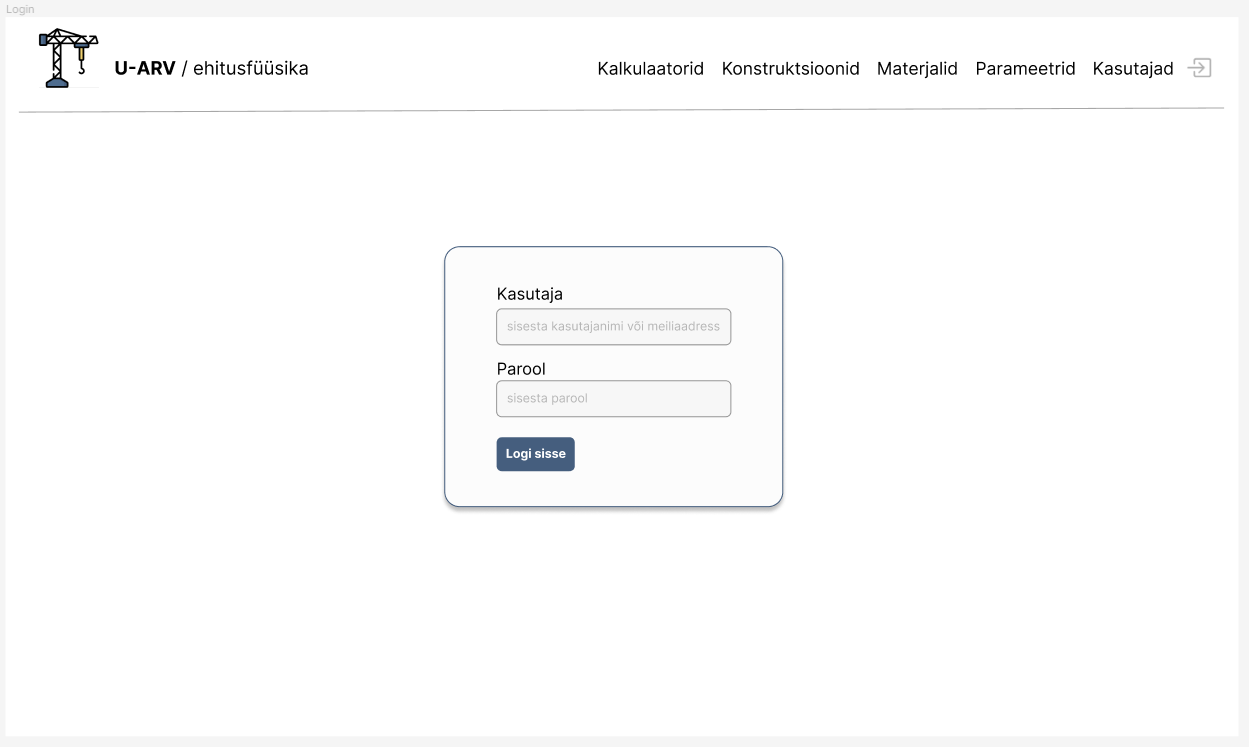
\includegraphics[width=.9\textwidth]{figures/interface_desing/ap_desing_login.png}
    \caption[Kasutajaliidese disaain: sisselogimise vorm]{\textit{Sisselogimise vorm}}
    \label{fig:interface_design_login}
\end{figure}
\begin{figure}[ht]
    \centering
    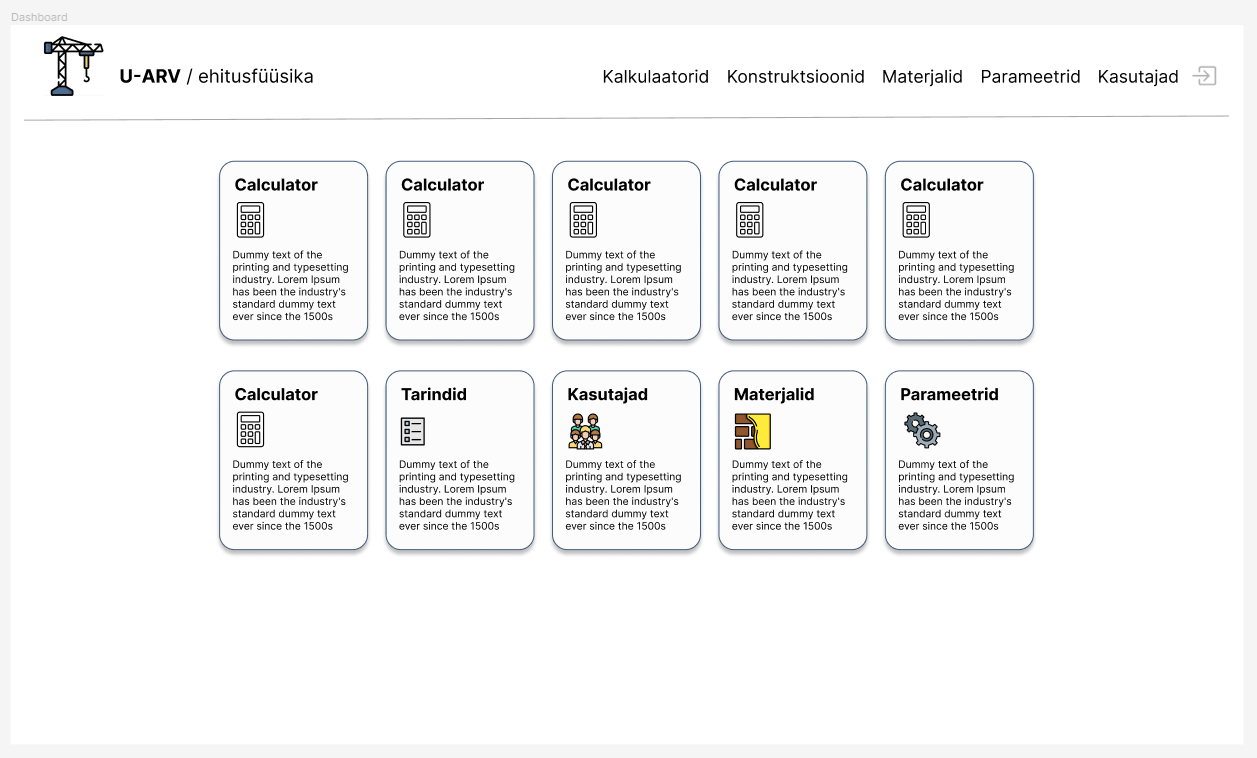
\includegraphics[width=.9\textwidth]{figures/interface_desing/ap_desing_dashboard.png}
    \caption[Kasutajaliidese disaain: pealeht]{\textit{Pealeht}}
    \label{fig:interface_design_dashboard}
\end{figure}
\begin{figure}[ht]
    \centering
    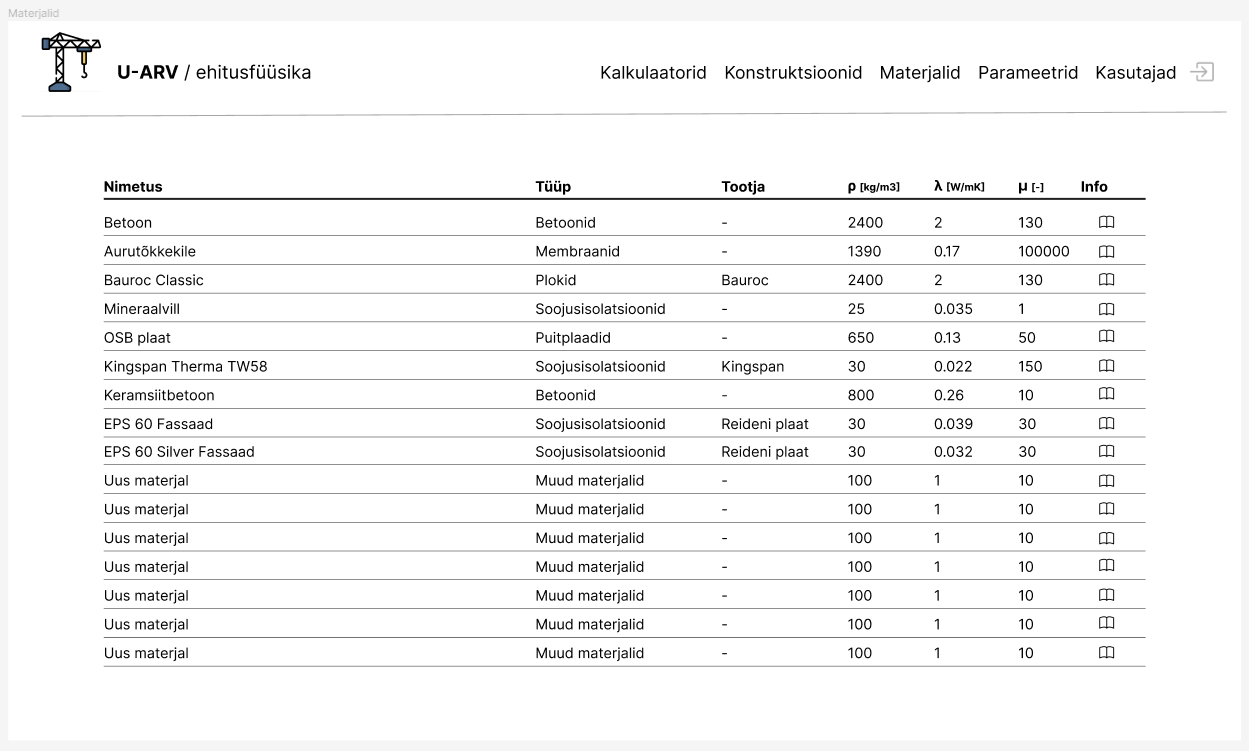
\includegraphics[width=.9\textwidth]{figures/interface_desing/ap_desing_materials.png}
    \caption[Kasutajaliidese disaain: materjalide nimekiri]{\textit{Materjalide nimekiri}}
    \label{fig:interface_design_materials}
\end{figure}
\begin{figure}[ht]
    \centering
    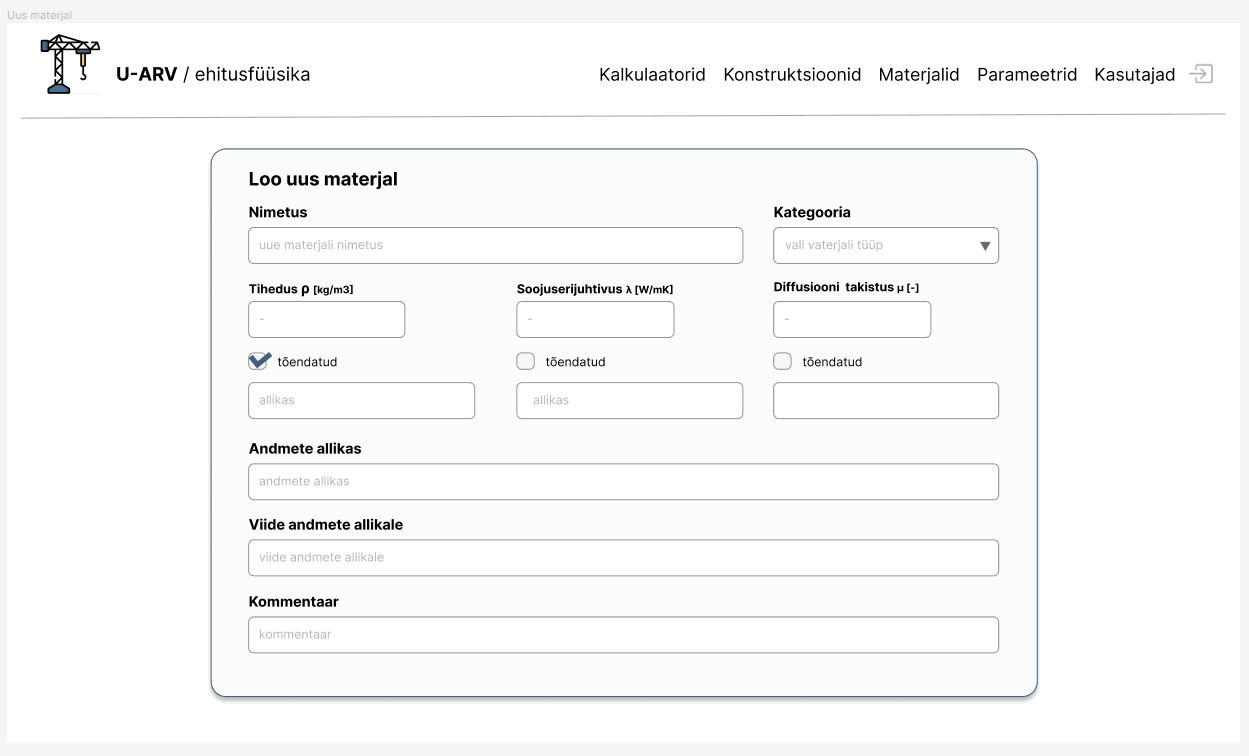
\includegraphics[width=.9\textwidth]{figures/interface_desing/ap_desing_addmaterial.png}
    \caption[Kasutajaliidese disaain: materjali lisamise vorm]{\textit{Materjali lisamise vorm}}
    \label{fig:interface_design_addmaterial}
\end{figure}
\begin{figure}[ht]
    \centering
    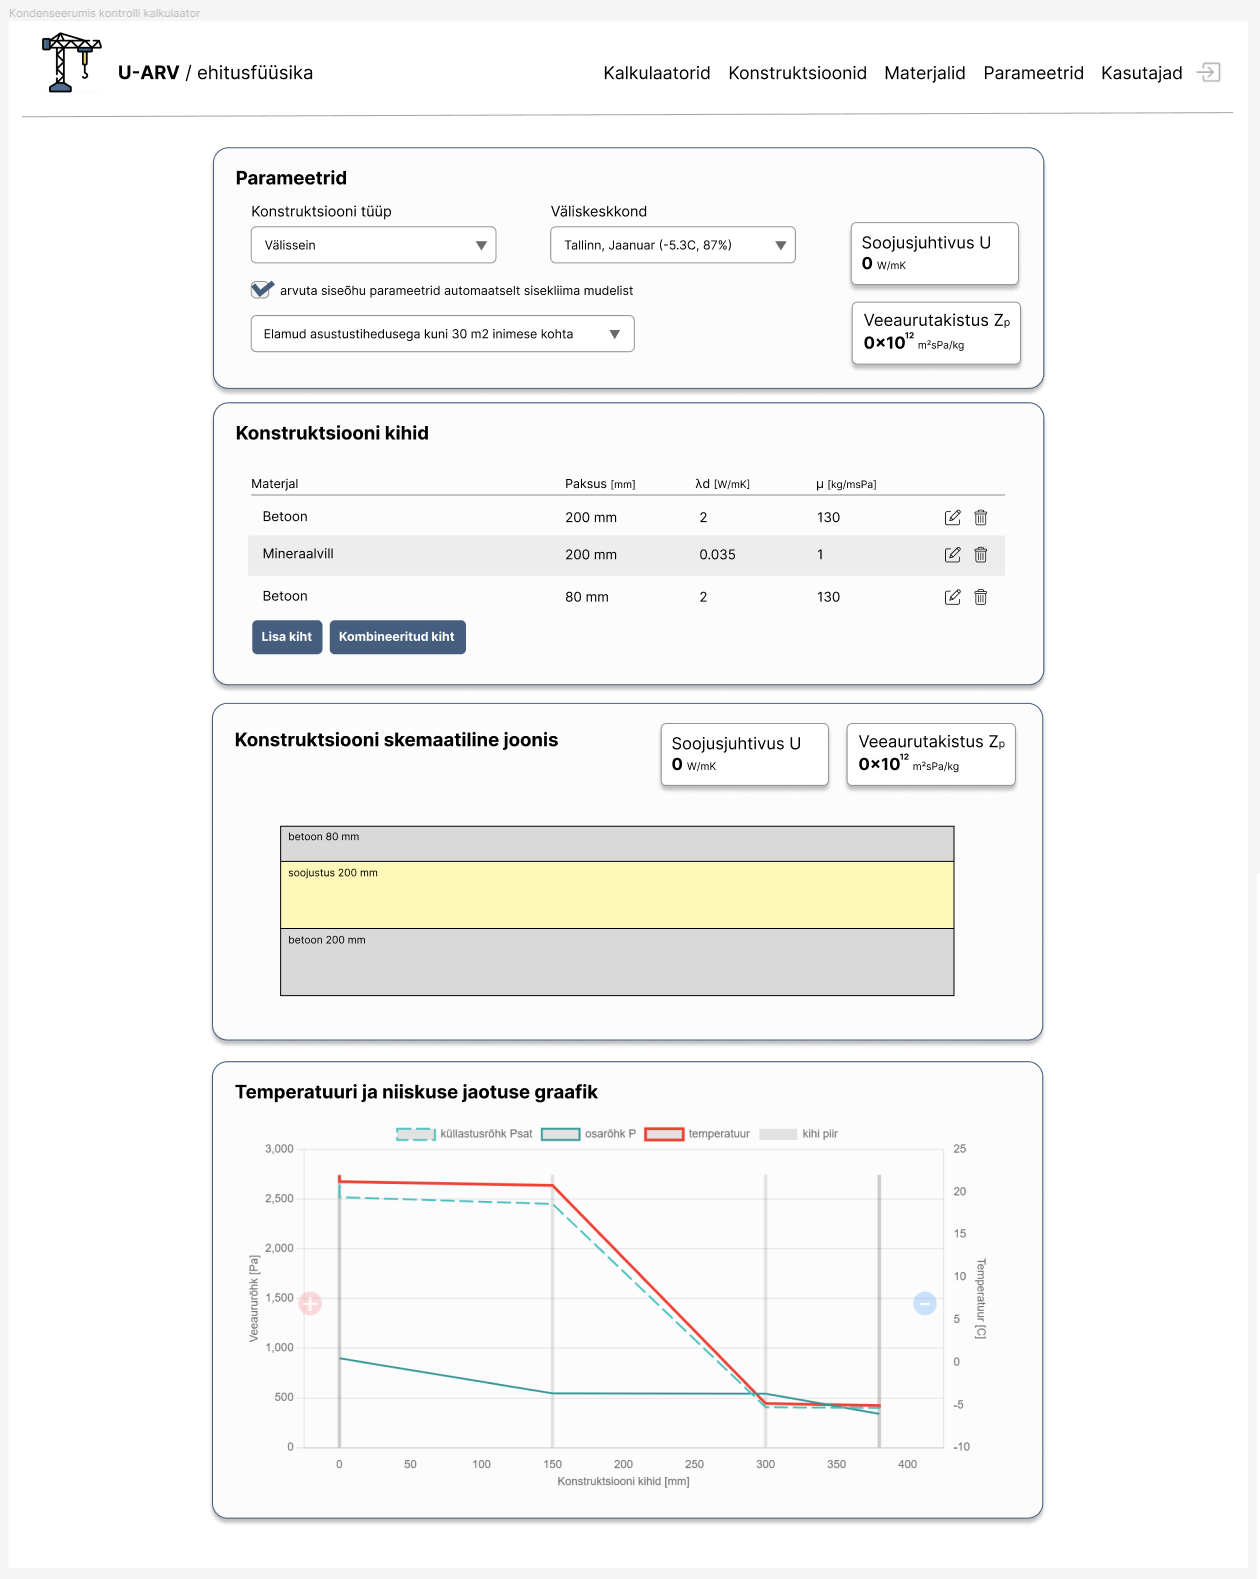
\includegraphics[width=.9\textwidth]{figures/interface_desing/ap_desing_calculator.png}
    \caption[Kasutajaliidese disaain: kalkulaatori vaade]{\textit{Kalkulaatori vaade}}
    \label{fig:interface_design_calculator}
\end{figure}








%\clearpage
%\phantomsection
%\addcontentsline{toc}{chapter}{Lisa 3 -- Something Else}\label{chapter:appendix-something-else}
%\chapter*{Lisa 3 -- Something Else}
%\textbf{Pythagorean theorem}
\begin{equation}
x^n + y^n = z^n
\end{equation}

\textbf{Normal distribution}%
\begin{equation}
P(x) = \frac{1}{{\sigma \sqrt {2\pi } }}e^{{{ - \left( {x - \mu } \right)^2 } \mathord{\left/ {\vphantom {{ - \left( {x - \mu } \right)^2 } {2\sigma ^2 }}} \right. \kern-\nulldelimiterspace} {2\sigma ^2 }}}
\end{equation}


\end{document}